%%
% BIThesis 本科毕业设计论文模板 —— 使用 XeLaTeX 编译 The BIThesis Template for Undergraduate Thesis
% This file has no copyright assigned and is placed in the Public Domain.
% Compile with: xelatex -> biber -> xelatex -> xelatex
%%

% 请勿删除下面两行注释，以免影响编译。
% !TeX program = xelatex
% !BIB program = biber


% 开启盲审格式 blindPeerReview=true (如：[type=bachelor,blindPeerReview=true])

\documentclass[type=bachelor]{bithesis}

% 此处仅列出常用的配置。全部配置用法请见「bithesis.pdf」手册。
\BITSetup{
  cover = {
    % 封面需要「北京理工大学」字样图片，如无必要请勿修改该项。
    headerImage = images/header.pdf,
    % 封面标题需要“华文细黑”，如无必要请勿修改该项。
    xiheiFont = STXIHEI.TTF,
    % 可用以下参数自定义封面日期。
    % date = 1955年11月,
  },
  info = {
    % 想要删除某项封面信息，直接删除该项即可。
    % 想要让某项封面信息留空（但是保留下划线），请传入空白符组成的字符串，如"{~}"。
    % 如需要换行，则用 “\\” 符号分割。
    title = 自重组轮足机器人链式系统协同控制,
    titleEn = {Cooperative Control of Chain-Structured Self-Reconfigurable Wheel-Legged Robotic Systems},
    school = 自动化学院,
    major = 自动化（徐特立英才班）,
    class = 06212202,
    author = 晋浩楠,
    studentId = 1120223117,
    supervisor = 宋文杰,
    keywords = {自重组轮足机器人；链式系统；协同控制；分布式模型预测控制；自抗扰控制},
    keywordsEn = {self-reconfigurable wheel-legged robot; chain-structured system; cooperative control; distributed model predictive control; active disturbance rejection control},
    % 如果你的毕设为校外毕设，请将下面这一行语句解除注释（删除第一个百分号字符）并填写你的校外毕设导师名字
    % externalSupervisor = 左偏树,
  },
  style = {
    % 开启 Windows 平台下的中易宋体伪粗体。
    % windowsSimSunFakeBold = true,
    %
    % 开启该选项后，将用 Times New Roman 的开源字体 TeX Gyre Termes 作为正文字体。
    % 这个选项适用于以下情况：
    % 1. 不想在系统中安装 Times New Roman。
    % 2. 在 Linux/macOS 下遇到 `\textsc` 无法正常显示的问题。
    % betterTimesNewRoman = true,
  },
  misc = {
    % 微调表格行间距
    tabularRowSeparation = 1.25,
  },
}

% 这份模板提供了代码块示例，采用 listings 宏包及其预定义样式。
% 使用代码块时，也可选用自己的喜欢的其他宏包，如 minted：https://bithesis.bitnp.net/faq/minted.html
% 如果不需要，直接删除即可。
\usepackage{listings}
\usepackage{graphicx}
\usepackage{placeins}
\usepackage{tikz}
\usetikzlibrary{arrows.meta,positioning,calc,fit}


% 大部分关于参考文献样式的修改，都可以通过此处的选项进行配置。
% 详情请搜索「biblatex-gb7714-2015 文档」进行阅读。
\usepackage[
  backend=biber,
  style=gb7714-2015,
  gbalign=gb7714-2015,
  gbnamefmt=lowercase,
  gbpub=false,
  doi=false,
  url=false,
  eprint=false,
  isbn=false,
]{biblatex}

% 参考文献引用文件位于 misc/ref.bib
\addbibresource{misc/ref.bib}

% 若要按计算机学院要求，添加“北京理工大学”水印，请参考
% https://bithesis.bitnp.net/faq/watermark.html

% 文档开始
\begin{document}

% 标题页面：如无特殊需要，本部分无需改动
\MakeCover

% 原创性声明：盲审结束前无需改动
% 后续添加签名时，可考虑先用 Word 制作再覆盖 misc/1_originality.pdf。
% 不过如无特殊需要，本部分的代码仍无需改动。
\begin{blindPeerReview}
  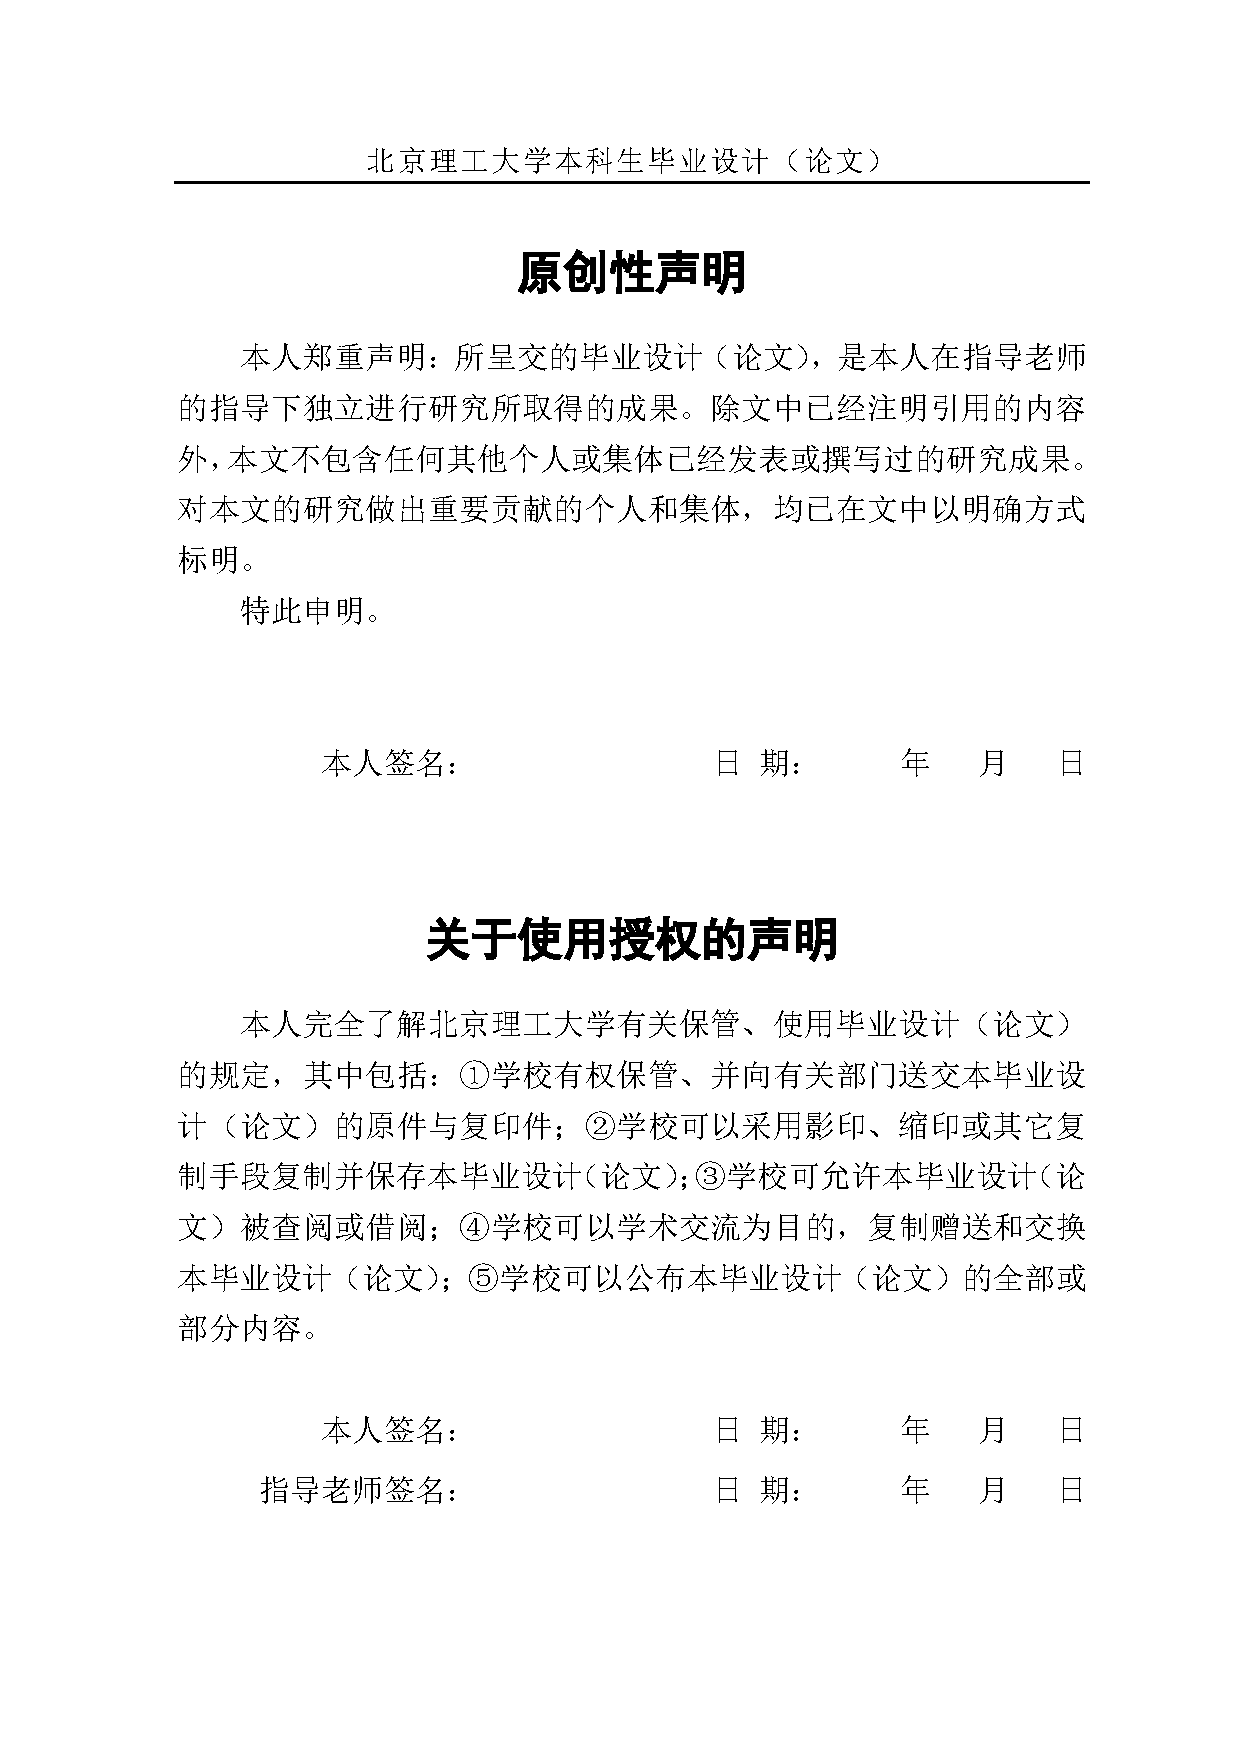
\includepdf{misc/1_originality.pdf}\newpage
\end{blindPeerReview}
% \input{misc/1_originality.tex}

% 前置内容定义
\frontmatter
% 摘要：在相应 TeX 文件撰写
%%
% BIThesis 本科毕业设计论文模板 —— 使用 XeLaTeX 编译 The BIThesis Template for Undergraduate Thesis
% This file has no copyright assigned and is placed in the Public Domain.
%%

% 中英文摘要章节
\begin{abstract}
% 中文摘要正文从这里开始
自重组轮足机器人兼具轮式移动效率、腿式姿态调节能力与模块化重构特性，在复杂地形通过、协同运输和多机器人系统扩展等场景中具有重要研究价值。针对多个轮足机器人单体通过铰接机构构成链式系统后存在的非完整运动约束、车体间强耦合以及单体平衡稳定性要求高等问题，本文围绕链式自重组轮足机器人协同控制方法展开研究。

首先，依据单体轮足机器人机构特征建立腿部运动学模型，推导关节空间与等效腿长、腿摆角之间的映射关系，并基于虚拟模型控制方法建立腿部支撑力、摆杆力矩与关节驱动力矩之间的等效关系。其次，针对尾部辅助机构在离地与触地两类支撑工况下对机体动力学的影响，建立单体机器人动力学模型，并在平衡点附近线性化得到状态空间表达；在此基础上设计线性二次型调节器，实现对机体姿态、腿部摆角、前向运动状态和尾部姿态的综合反馈控制。针对腿长变化导致模型参数变化的问题，进一步采用参数化增益拟合方法描述控制器增益与构型参数之间的关系，以提高控制器对变构型过程的适应性。

在链式系统协同控制方面，本文根据相邻单体之间的铰接几何关系建立链式运动学约束模型，并由头车运动指令和各单体航向状态推导后续单体的期望速度传播关系。进一步地，构建分层协同控制框架：上层依据链式运动学模型生成满足几何约束的期望运动序列，下层通过单体平衡控制器实现对期望状态的稳定跟踪。该方法为后续引入分布式模型预测控制约束优化和鲁棒扰动补偿提供了理论基础。研究结果表明，所建立的建模与控制框架能够统一描述单体平衡控制与链式协同运动之间的关系，为链式自重组轮足机器人实机控制和性能优化提供了可行技术途径。

\end{abstract}

% 如需手动控制换行连字符位置，可写 aa\-bb，详见
% https://bithesis.bitnp.net/faq/hyphen.html

% 英文摘要章节
\begin{abstractEn}
% 英文摘要正文从这里开始
Self-reconfigurable wheel-legged robots combine the efficiency of wheeled locomotion, the posture-adjusting capability of legged mechanisms, and the structural flexibility of modular robotic systems. They are therefore promising for rough-terrain traversal, cooperative transportation, and scalable multi-robot applications. This thesis investigates cooperative control of a chain-structured self-reconfigurable wheel-legged robotic system, in which multiple balancing wheel-legged modules are connected through articulated joints. The main challenges arise from nonholonomic motion constraints, strong inter-module coupling, and the stability requirement of each balancing module.

First, the kinematic model of the leg mechanism is established according to the wheel-legged structure, and the mapping between the joint coordinates and the equivalent leg length and leg swing angle is derived. Based on virtual model control, the relationship between the virtual supporting force, hip torque, and joint actuation torque is formulated. Then, considering the influence of the tail-assisted mechanism under different contact conditions, a dynamic model of the single module is developed and linearized around the equilibrium point. A linear quadratic regulator is designed to stabilize the body posture, leg swing motion, longitudinal motion, and tail posture. To account for configuration variation caused by changes in leg length, a parameterized gain fitting method is introduced to describe the dependence of the feedback gain on structural parameters.

For cooperative control of the chain-structured system, the geometric constraints between adjacent modules are analyzed, and the velocity propagation relationship from the leading module to the following modules is derived from the articulated kinematic model. A hierarchical cooperative control framework is further constructed: the upper layer generates feasible reference motion sequences satisfying the chain constraints, while the lower layer tracks the desired states through the balancing controller of each module. The proposed modeling and control framework provides a unified description of single-module stabilization and chain-level cooperative motion, and lays a theoretical foundation for further constrained optimization using distributed model predictive control and robust disturbance compensation.
\end{abstractEn}


\MakeTOC

% 正文开始
\mainmatter

% 在这里引用各章 TeX 文件，按需添加
% 模板原示例章节保留在 chapters/1_chapter1.tex 和 chapters/2_chapter2.tex 中，
% 其中包含正文、图、表、公式、代码块等格式要求提示词；需要查看格式示例时，可临时取消下面两行注释。
% \input{chapters/1_chapter1.tex}
% \input{chapters/2_chapter2.tex}

\chapter{绪论}

\section{研究背景与意义}
移动机器人是机器人学、自动控制、机械电子工程和人工智能等学科交叉发展的重要研究方向，在复杂环境探测、灾害救援、工业巡检、协同运输和特种作业等领域具有广泛应用价值\cite{siegwart2011introduction,corke2017robotics}。传统移动机器人按照运动机构形式通常可分为轮式、履带式和腿式等类型。轮式机器人结构简单、运动效率高、控制实现相对容易，适合在结构化或半结构化道路环境中快速移动；履带式机器人具有较强地形适应能力和越障能力，但能耗、转向阻力和机构磨损相对较大；腿式机器人能够通过离散支撑点适应复杂地形，具备较好的跨越障碍和姿态调节能力，但系统自由度多、动力学模型复杂、控制难度和能量消耗较高。因此，如何在移动效率、复杂地形适应能力、系统稳定性和控制实现复杂度之间取得平衡，是移动机器人平台设计与控制研究中的重要问题。

轮足机器人通过在腿式机构末端引入轮式驱动，将轮式运动的高效率与腿式机构的姿态调节能力相结合。与纯轮式平台相比，轮足机器人能够通过腿长变化、机体姿态调节和支撑位置调整适应坡面、坑洼、台阶和松软地面等非结构化环境；与纯腿式平台相比，其在平坦或连续地面上可利用轮式滚动实现更高速度和更低能耗的运动。Roller-Walker、Wheel Transformer、Ascento 以及带轮足式四足平台等典型研究表明，轮腿复合移动方式是兼顾机动性、通过性和工程可实现性的有效技术路径\cite{endo1999roller,kim2014wheel,klemm2019ascento,bjelonic2021whole,grandia2019feedback}。

自重构机器人则强调机器人系统能够根据任务需求、环境条件或故障状态改变自身结构形态。模块化自重构机器人通常由多个具有感知、计算、驱动和连接能力的模块组成，通过标准化机械接口和分布式控制方式实现模块间组合、分离和重构\cite{fukuda1988dynamically,chirikjian1994kinematics,yim2000polybot,murata2002mtran,yim2007modular,murata2007self}。与固定构型机器人相比，自重构机器人具有更高的结构柔性、任务适应性和系统冗余性。将轮足移动能力与模块化自重构能力相结合，有望构建一种兼具高效移动、姿态调节、构型重组和协同作业能力的新型移动机器人系统。

本文研究对象为链式自重组轮足机器人系统。该系统由多个具备独立平衡移动能力的轮足机器人单体通过铰接机构串联组成。单体层面上，机器人具有轮式倒立摆特性和腿部可变构型特性，控制器需要同时处理机体俯仰稳定、腿长调节、速度跟踪和尾部辅助机构等问题；链式系统层面上，相邻单体之间存在铰接几何约束和速度一致约束，任一单体的运动都会对相邻单体产生影响，系统整体表现出明显的非完整约束、强耦合和多体协同特征。与常规多机器人队形控制不同，链式系统中的各单体并非仅通过通信或相对位姿保持形成队形，而是通过物理铰接结构构成一个受约束的多体系统。

链式自重组轮足机器人在复杂地形通过、狭窄空间穿越、协同运输和多模块任务扩展等场景中具有潜在应用价值。例如，在沙地、碎石地、楼梯、沟壑或障碍密集环境中，链式构型能够通过多个单体的支撑分布提高整体稳定性；在载荷运输任务中，多个单体可通过机械连接共同承担负载；在特殊环境探测中，系统可根据通道形状或任务需求改变链式姿态和运动方式。上述应用对系统建模与控制提出了新的要求：一方面，需要建立能够描述单体轮足机构、尾部辅助机构和欠驱动平衡特性的动力学模型；另一方面，需要建立能够反映相邻单体铰接约束、速度一致关系和链式构型变化规律的协同运动模型。

\tikzset{
  ctrlBlock/.style={
    draw,
    rounded corners=2pt,
    align=center,
    minimum height=8mm,
    minimum width=24mm,
    inner xsep=4pt,
    inner ysep=3pt,
    font=\small
  },
  ctrlSmall/.style={
    draw,
    rounded corners=2pt,
    align=center,
    minimum height=7mm,
    minimum width=20mm,
    inner xsep=3pt,
    inner ysep=2pt,
    font=\footnotesize
  },
  ctrlSum/.style={
    draw,
    circle,
    inner sep=0pt,
    minimum size=5.5mm,
    font=\small
  },
  ctrlGroup/.style={
    draw,
    dashed,
    rounded corners=3pt,
    inner sep=6pt
  },
  ctrlArrow/.style={
    -{Latex[length=2.2mm]},
    line width=0.45pt
  },
  ctrlDashArrow/.style={
    -{Latex[length=2.2mm]},
    dashed,
    line width=0.45pt
  }
}


\begin{figure}[htbp]
  \centering
  \resizebox{0.98\textwidth}{!}{%
  \begin{tikzpicture}
    \node[ctrlBlock, minimum width=31mm] (mobile) at (0,0) {移动机器人\\平台需求};
    \node[ctrlBlock, minimum width=31mm] (wheelleg) at (4.0,1.4) {轮足复合\\高效移动/越障};
    \node[ctrlBlock, minimum width=31mm] (reconfig) at (4.0,0) {模块化自重构\\构型适应/冗余};
    \node[ctrlBlock, minimum width=31mm] (multi) at (4.0,-1.4) {多机器人协同\\信息交互/分布式};

    \node[ctrlBlock, minimum width=36mm] (target) at (8.4,0) {链式自重组\\轮足机器人系统};
    \node[ctrlSmall, minimum width=25mm] (single) at (12.2,1.35) {单体平衡\\变腿长控制};
    \node[ctrlSmall, minimum width=25mm] (chain) at (12.2,0) {铰接约束\\链式运动学};
    \node[ctrlSmall, minimum width=25mm] (coop) at (12.2,-1.35) {分层协同\\DMPC/ADRC};

    \draw[ctrlArrow] (mobile) -- (wheelleg);
    \draw[ctrlArrow] (mobile) -- (reconfig);
    \draw[ctrlArrow] (mobile) -- (multi);
    \draw[ctrlArrow] (wheelleg) -- (target);
    \draw[ctrlArrow] (reconfig) -- (target);
    \draw[ctrlArrow] (multi) -- (target);
    \draw[ctrlArrow] (target) -- (single);
    \draw[ctrlArrow] (target) -- (chain);
    \draw[ctrlArrow] (target) -- (coop);

    \node[ctrlGroup, fit=(wheelleg)(reconfig)(multi), label={[font=\footnotesize]above:相关研究方向}] {};
    \node[ctrlGroup, fit=(single)(chain)(coop), label={[font=\footnotesize]above:本文关注问题}] {};
  \end{tikzpicture}
  }%
  \caption{链式自重组轮足机器人相关研究方向与本文问题定位}
  \label{fig:ch1_research_landscape}
\end{figure}


因此，开展链式自重组轮足机器人协同控制研究具有以下意义。第一，从理论层面看，该问题融合了轮足机器人平衡控制、非完整系统建模、多体约束动力学和多机器人协同控制等内容，有助于深化对变构型轮足系统运动机理的理解。第二，从方法层面看，将单体稳定控制与链式协同控制分层处理，有助于降低高维强耦合系统的控制复杂度，并为分布式模型预测控制、鲁棒扰动补偿等方法在链式机器人系统中的应用提供基础。第三，从工程层面看，建立可实时实现的单体控制器和链式期望运动生成方法，有助于推动自重组轮足机器人由单体平衡实验向多体协同运动和复杂场景应用发展。

\section{国内外研究现状}
\subsection{自重组轮足机器人研究现状}
自重构机器人研究最早可追溯到可动态重构机械系统和模块化机器人系统。早期 CEBOT 系统较早体现了机器人模块通过连接组合形成不同功能结构的思想\cite{fukuda1988dynamically}。随后，针对 metamorphic robot 的构型运动学分析为模块化机器人构型描述和重构运动奠定了理论基础\cite{chirikjian1994kinematics}。

随后，PolyBot、CONRO、M-TRAN、SuperBot 等系统相继提出，推动了模块化自重构机器人从概念验证向实际机构、通信接口、重构控制和多模态运动方向发展\cite{yim2000polybot,castano2000conro,murata2002mtran,salemi2006superbot}。Yim 等系统总结了模块化自重构机器人在可重构性、鲁棒性和多任务适应性方面的优势，同时指出模块连接机构设计、构型识别、重构规划和分布式控制仍是该领域的重要挑战\cite{yim2007modular}。Murata 和 Kurokawa 从系统结构、运动方式和应用场景等方面进行综述，指出模块化机器人可通过改变连接关系实现结构和功能的动态适应\cite{murata2007self}。

\begin{figure}[htbp]
  \centering
  \begin{minipage}[t]{0.47\textwidth}
    \centering
    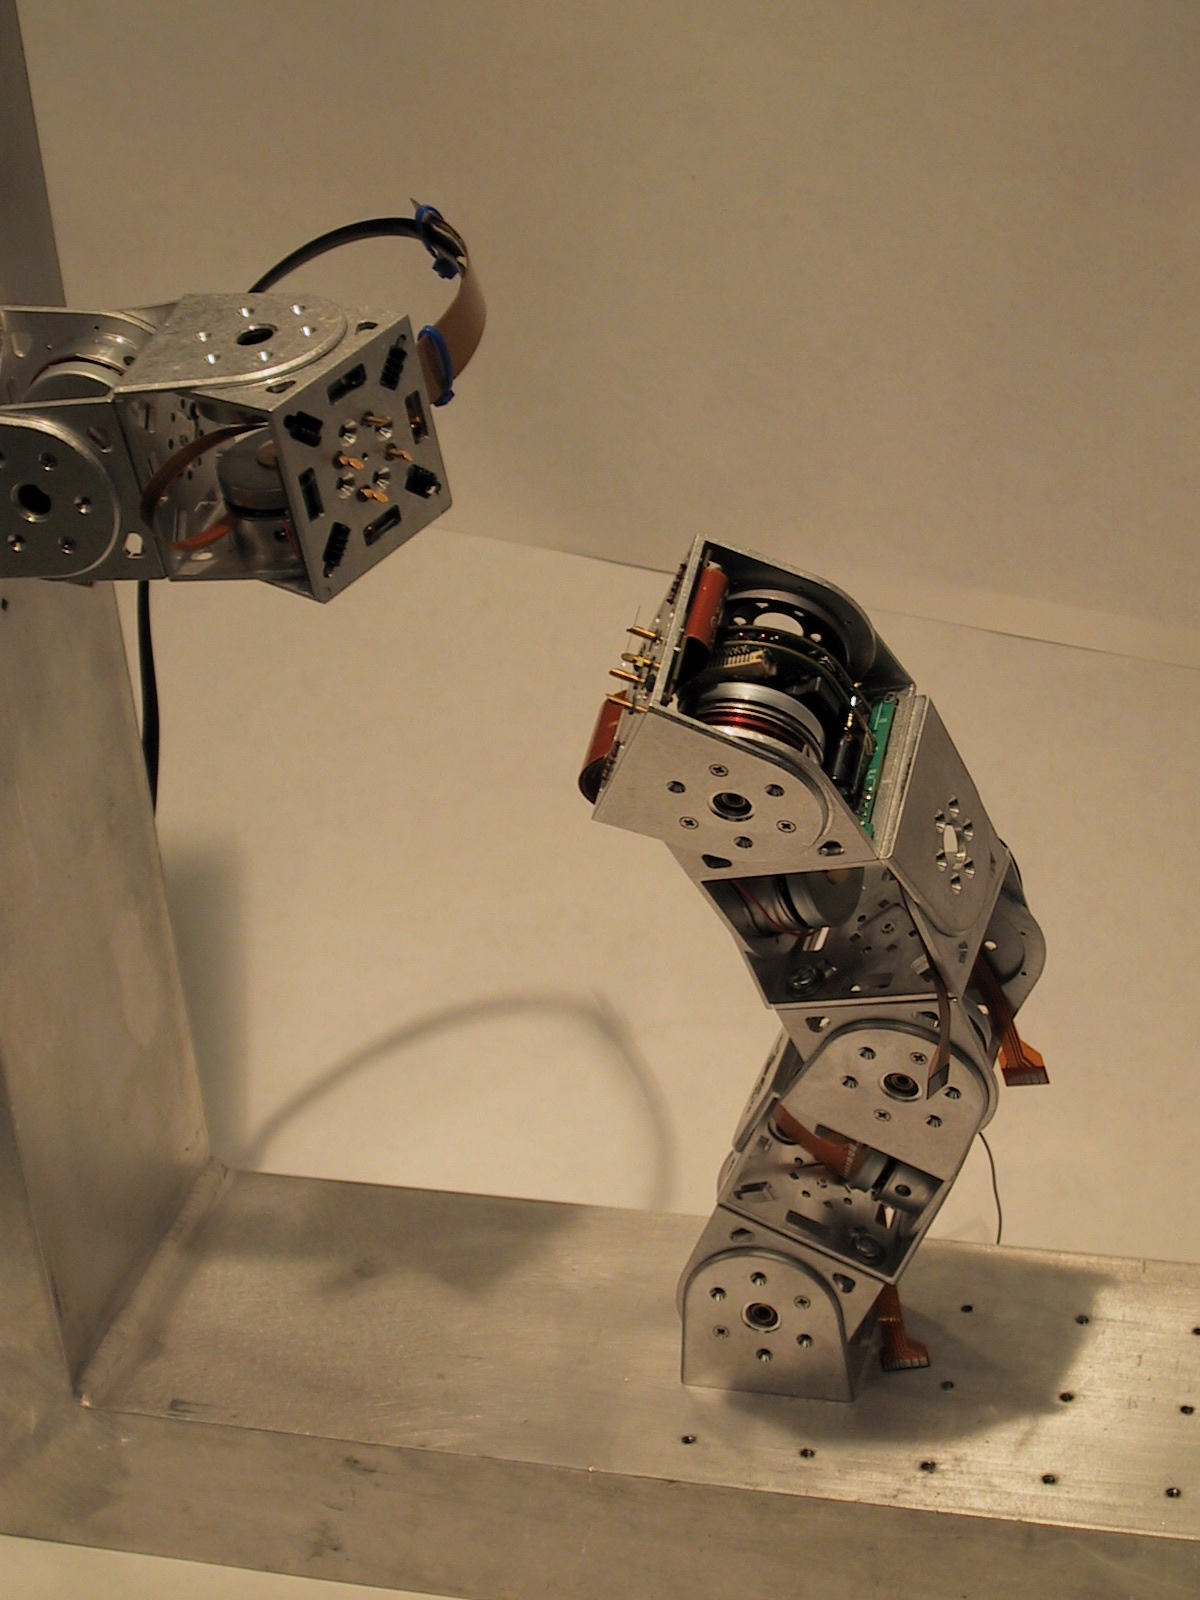
\includegraphics[height=0.22\textheight,keepaspectratio]{images/literature/polybot_g3.jpg}\\
    \small (a) PolyBot 模块化自重构机器人
  \end{minipage}
  \hfill
  \begin{minipage}[t]{0.47\textwidth}
    \centering
    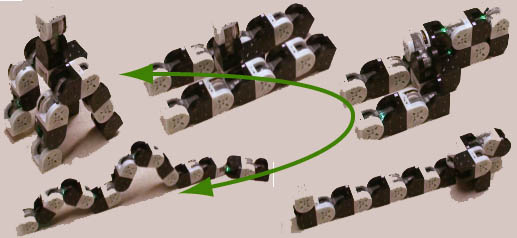
\includegraphics[width=\textwidth,height=0.22\textheight,keepaspectratio]{images/literature/mtran_iii.jpg}\\
    \small (b) M-TRAN III 多构型运动示例
  \end{minipage}
  \caption{典型模块化自重构机器人实物示例（图片来源：Wikimedia Commons）}
  \label{fig:ch1_self_reconfigurable_robots}
\end{figure}

从构型特征看，自重构机器人通常可分为链式、晶格式和混合式等类型。链式结构模块通过串联连接形成蛇形、环形、腿式或多臂结构，具有较强构型表达能力和运动灵活性；晶格式结构模块通常在规则空间网格中移动和重排，便于形成稳定三维结构；混合式结构则兼具链式和晶格式特点\cite{yim2007modular,chennareddy2017modular}。本文所研究的链式自重组轮足机器人属于具有主动移动能力的链式连接系统，其特点在于每个模块本身并非被动连接单元，而是具有独立平衡移动能力的轮足机器人单体。因此，该系统既不同于传统模块化自重构机器人中以重构规划为核心的问题，也不同于普通多机器人系统中各机器人相互独立运动的队形控制问题，而是需要同时考虑单体平衡稳定和链式几何约束。

轮足机器人方面，早期 Roller-Walker 采用腿端被动轮实现轮式与腿式运动模式切换，验证了腿轮复合机构在能量效率和地形适应性方面的优势\cite{endo1999roller}。Kim 等提出 Wheel Transformer，通过可变形轮结构在平地滚动和越障运动之间切换，提高了小型移动平台对障碍环境的适应能力\cite{kim2014wheel}。Ascento 采用两轮平衡加腿部跳跃结构，在保持平地快速移动能力的同时具备一定跳跃越障能力\cite{klemm2019ascento}。近年来，带轮足式四足机器人进一步将轮式滚动约束与腿式全身控制结合，通过模型预测控制、接触规划和全身动力学优化实现高速、灵活的多地形运动\cite{bjelonic2021whole,geilinger2020computational,grandia2019feedback}。这些研究表明，轮足机器人能够有效结合轮式和腿式运动优势，但同时也带来了机构自由度增加、动力学耦合增强和控制器实时性要求提高等问题。

在单体控制方法方面，轮足平衡机器人常可抽象为轮式倒立摆或带可变腿长的欠驱动系统。针对该类系统，常见控制方法包括 PID 控制、线性二次型调节器、滑模控制、虚拟模型控制、模型预测控制和全身动力学控制等。Raibert 关于动态平衡腿式机器人的研究为足式机器人运动控制提供了重要思想\cite{raibert1986legged}；Pratt 等提出的虚拟模型控制方法通过构造虚拟弹簧、阻尼和力元件，将高层期望力映射到底层关节力矩，具有直观性和工程可实现性\cite{pratt2001virtual}；LQR 方法则可在系统平衡点附近根据线性化模型构造状态反馈控制律，兼顾状态调节性能和输入能量约束\cite{anderson1990optimal,kirk1970optimal}。对于本文所研究的单体轮足机器人，腿长变化、尾部辅助机构接触状态变化和地面扰动会导致模型参数发生变化，单一固定增益控制器难以覆盖全部运动工况。因此，结合参数化增益拟合和鲁棒扰动补偿的控制设计具有实际意义。

综上，现有自重构机器人研究主要关注模块机构、重构规划和分布式构型控制，现有轮足机器人研究主要关注单体机构设计、动态运动和复杂地形适应能力，而将多个具备平衡移动能力的轮足单体通过铰接结构组成链式系统后的协同控制问题仍有进一步研究空间。该问题的关键不只是让每个单体保持稳定运动，还需要保证相邻单体在铰接点处满足位置和速度一致性，从而避免链式构型误差累积和运动约束冲突。

\subsection{多机器人协同控制研究现状}
多机器人协同控制是多智能体系统和移动机器人领域的重要研究方向，其核心目标是通过信息交互和控制协调，使多个机器人在完成个体任务的同时实现群体层面的期望行为。常见研究内容包括一致性控制、领航-跟随控制、队形控制、协同路径规划、任务分配和分布式优化等\cite{ren2007information,olfati2007consensus,ren2008distributed,liu2018survey}。Ren 等对多车辆协同控制中的信息一致性问题进行了系统总结，指出局部信息交互是实现多机器人群体协同的重要基础\cite{ren2007information}。Olfati-Saber 等从图论和网络系统角度建立了多智能体一致性与协同控制理论框架，为分析网络拓扑、通信延迟和信息流方向对协同行为的影响提供了理论工具\cite{olfati2007consensus}。

然而，链式自重组轮足机器人与一般多机器人队形系统存在显著差异。一般多机器人系统中，机器人之间多通过通信、视觉或相对定位保持队形，个体之间通常不存在刚性机械连接；而链式系统中，相邻单体通过铰接机构连接，系统必须满足铰接点位置一致和速度一致约束。该类约束使得后车运动不再是独立规划问题，而是受到前车速度、航向角、铰接角和几何参数的共同影响。这与非完整移动机器人和铰接车辆系统中的运动约束问题具有一定相似性\cite{murray1993nonholonomic,campion1996structural,laumond1998robot,lamiraux2001smooth}。上述研究为链式机器人系统的运动学约束建模提供了重要参考。

\begin{figure}[htbp]
  \centering
  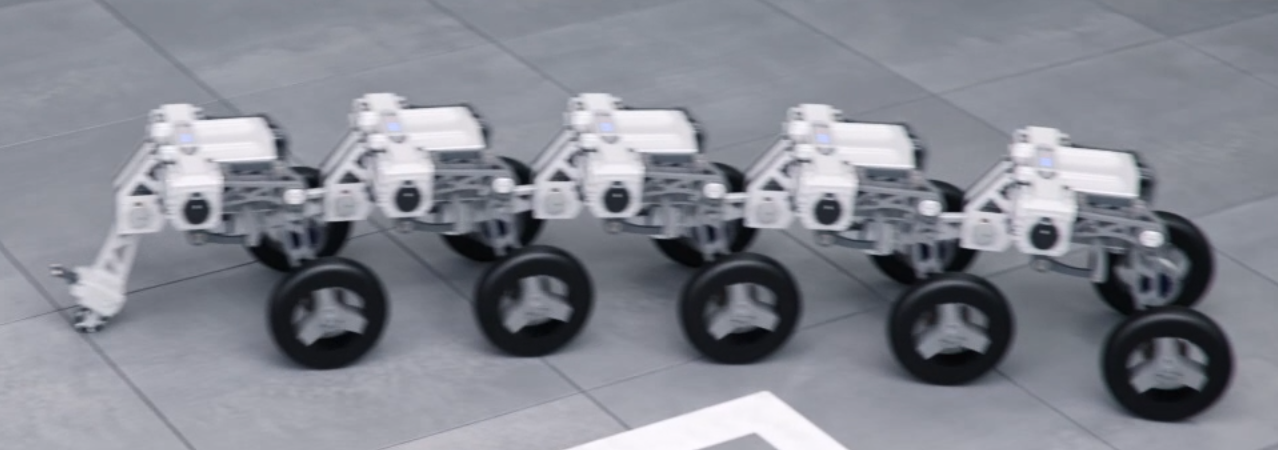
\includegraphics[width=0.92\textwidth]{images/literature/image.png}
  \caption{链式铰接轮足机器人模型示例}
  \label{fig:ch1_articulated_vehicle}
\end{figure}

模型预测控制由于能够显式处理系统约束、多变量耦合和有限时域优化问题，近年来被广泛应用于移动机器人、车辆系统和多机器人协同控制中\cite{camacho2007model,rawlings2017model,mayne2000constrained}。MPC 通过在每个采样时刻求解有限时域优化问题，并仅执行当前时刻最优控制输入，能够根据最新状态滚动修正未来控制序列。对于链式轮足系统而言，MPC 的优势在于可以在预测时域内同时考虑速度跟踪误差、铰接角约束、输入幅值约束和输入变化率约束，从而提高链式构型保持能力和运动平滑性。

随着机器人数量增加，集中式 MPC 会面临优化变量维度高、求解时间长和通信负担重等问题。分布式模型预测控制通过将全局优化问题分解为多个局部优化问题，使每个机器人仅基于自身和邻近机器人的状态进行滚动优化，从而提高系统可扩展性和实时性\cite{dunbar2006distributed,christofides2013distributed,farina2012distributed}。Dunbar 和 Murray 将分布式滚动时域控制应用于多车辆队形稳定问题，证明了在一定条件下系统可稳定到目标邻域\cite{dunbar2006distributed}。对于本文研究的链式系统，铰接约束天然具有局部相邻耦合特点，因此采用分布式 MPC 协调相邻单体的预测轨迹和控制输入具有较强合理性。

除协同层的预测控制外，单体层面的鲁棒性同样是链式系统稳定运行的关键。轮足机器人在实际运动中会受到地面摩擦变化、机体参数不确定性、轮地接触扰动、铰接传递力以及尾部辅助机构状态切换等影响。自抗扰控制通过扩张状态观测器估计系统总扰动，并在控制律中进行补偿，能够在模型不精确和外部扰动存在时提高系统鲁棒性\cite{han2009pid,gao2003scaling,huang2000analysis,guo2016active,sira2017active}。因此，在单体 LQR 平衡控制基础上引入 ADRC 扰动补偿，有助于增强链式系统在复杂地形和强耦合条件下的跟踪稳定性。

总体而言，现有多机器人协同控制和 MPC 研究为链式轮足系统提供了重要方法基础，但仍存在以下不足：第一，多数队形控制研究假设机器人之间没有刚性物理连接，难以直接处理铰接点位置和速度一致约束；第二，部分铰接车辆研究主要面向平面车辆或拖车系统，较少考虑轮足单体的欠驱动平衡和变腿长构型；第三，轮足机器人控制研究多集中于单体运动性能，对多个平衡轮足单体机械连接后的误差传播和协同控制关注不足；第四，单体平衡控制与链式协同控制之间的层级关系仍需进一步明确。基于上述问题，本文围绕链式自重组轮足机器人系统，建立单体轮足建模、链式运动学约束建模和分层协同控制框架，为后续实机控制和性能优化提供基础。

\section{本文主要研究内容}
本文以链式自重组轮足机器人为研究对象，围绕单体建模、基础平衡控制、链式运动学约束和协同控制优化等问题展开研究。主要研究内容如下。

第一，建立单体轮足机器人结构模型与腿部运动学模型。根据机器人单体的轮腿复合结构，定义机体坐标系、世界坐标系和腿部虚拟变量，分析四连杆腿部机构的几何约束关系，推导关节空间与等效腿长、腿摆角之间的映射关系。在此基础上，基于虚功原理建立虚拟腿空间广义力与关节驱动力矩之间的映射关系，为后续腿长调节、姿态控制和关节力矩分配提供运动学基础。

第二，建立单体轮足机器人的动力学模型并设计基础平衡控制器。针对尾部辅助机构离地和触地等典型工况，分析机体、腿部、轮端和尾部机构之间的受力关系，采用牛顿-欧拉方法建立单体动力学方程，并通过消去内部约束力得到适合控制器设计的动力学表达。在平衡点附近对系统进行线性化，建立状态空间模型，并基于线性二次型调节器设计单体平衡控制器。

第三，研究腿长变化和构型变化对单体控制器的影响。由于腿长变化会改变系统质量分布、几何参数和线性化模型，固定反馈增益难以在较大构型范围内保持一致控制性能。为提高控制器对变构型过程的适应性，本文在不同腿长组合下计算平衡点和 LQR 反馈增益，并采用参数化拟合方法描述控制器增益与左右腿长之间的关系。

第四，建立链式系统运动学约束模型。针对多个单体通过铰接机构串联形成的链式结构，分析相邻单体之间的铰接角关系、位置一致约束和速度一致约束。根据平面刚体运动学，推导由前车速度、前车角速度和相邻航向角关系确定后车期望线速度与角速度的运动学模型。该模型能够描述头车运动指令向后续单体逐级传播的过程，是链式系统期望运动序列生成和协同控制器设计的基础。

第五，构建链式系统分层协同控制框架。针对单体平衡控制与链式几何约束之间的耦合问题，本文采用分层控制思想：上层协同控制器根据链式运动学模型生成满足铰接约束的期望速度和姿态序列，下层单体控制器根据期望状态完成局部平衡控制和力矩分配。在此基础上，进一步讨论基于分布式模型预测控制的协同跟踪策略，将速度误差、铰接角误差、铰接点速度一致误差和输入变化率等纳入预测优化指标。

第六，研究基于 LQR-ADRC 的单体鲁棒控制扩展方法。针对模型误差、地面扰动、链式铰接耦合和尾部状态变化等因素对单体跟踪性能的影响，本文在 LQR 状态反馈基础上引入扩张状态观测器，将未建模动态和外部扰动视为总扰动进行估计，并将扰动估计量作为补偿项引入控制律，从而构成 LQR-ADRC 复合控制结构。

\tikzset{
  ctrlBlock/.style={
    draw,
    rounded corners=2pt,
    align=center,
    minimum height=8mm,
    minimum width=24mm,
    inner xsep=4pt,
    inner ysep=3pt,
    font=\small
  },
  ctrlSmall/.style={
    draw,
    rounded corners=2pt,
    align=center,
    minimum height=7mm,
    minimum width=20mm,
    inner xsep=3pt,
    inner ysep=2pt,
    font=\footnotesize
  },
  ctrlSum/.style={
    draw,
    circle,
    inner sep=0pt,
    minimum size=5.5mm,
    font=\small
  },
  ctrlGroup/.style={
    draw,
    dashed,
    rounded corners=3pt,
    inner sep=6pt
  },
  ctrlArrow/.style={
    -{Latex[length=2.2mm]},
    line width=0.45pt
  },
  ctrlDashArrow/.style={
    -{Latex[length=2.2mm]},
    dashed,
    line width=0.45pt
  }
}


\begin{figure}[htbp]
  \centering
  \resizebox{0.98\textwidth}{!}{%
  \begin{tikzpicture}
    \node[ctrlBlock] (task) at (0,0) {链式自重组\\轮足机器人};
    \node[ctrlBlock] (model) at (3.0,0) {单体/链式\\建模};
    \node[ctrlBlock] (single) at (6.0,0) {单体稳定\\控制};
    \node[ctrlBlock] (coop) at (9.0,0) {链式协同\\控制};
    \node[ctrlBlock] (exp) at (12.0,0) {实验验证\\与对比};

    \node[ctrlSmall] (kin) at (3.0,-1.35) {运动学约束};
    \node[ctrlSmall] (lqr) at (6.0,-1.35) {LQR 基础控制};
    \node[ctrlSmall] (dmpc) at (9.0,-1.35) {DMPC / ADRC};

    \draw[ctrlArrow] (task) -- (model);
    \draw[ctrlArrow] (model) -- (single);
    \draw[ctrlArrow] (single) -- (coop);
    \draw[ctrlArrow] (coop) -- (exp);
    \draw[ctrlArrow] (model) -- (kin);
    \draw[ctrlArrow] (single) -- (lqr);
    \draw[ctrlArrow] (coop) -- (dmpc);
    \draw[ctrlDashArrow] (exp.south) -- ++(0,-2.35) -| node[pos=0.28, below, font=\footnotesize] {性能评价与参数修正} (model.south);
  \end{tikzpicture}
  }%
  \caption{第 1 章研究内容与控制方案总体关系框图}
  \label{fig:ch1_control_route}
\end{figure}


\section{论文组织结构}
本文共分为五章，各章内容安排如下。

第一章为绪论。主要介绍链式自重组轮足机器人协同控制问题的研究背景与意义，综述自重组机器人、轮足机器人、多机器人协同控制、模型预测控制和自抗扰控制等相关研究现状，并说明本文主要研究内容与论文结构。

第二章为链式系统建模。首先介绍单体轮足机器人结构和坐标系定义，建立单体平面运动学模型和腿部四连杆机构运动学模型；随后基于虚拟模型控制思想推导虚拟腿空间广义力与关节力矩之间的映射关系；最后分析相邻单体的铰接结构与运动约束，建立链式系统运动学模型。

第三章为单机动力学分析与基础控制器设计。针对单体轮足机器人欠驱动、变构型和尾部辅助支撑等特点，建立单体动力学模型，并在平衡点附近线性化得到状态空间表达；在此基础上设计 LQR 基础平衡控制器，并结合腿长变化讨论参数化增益拟合方法。

第四章为协同控制器优化方案。首先分析单体 LQR 控制器在链式连接场景下面临的局限性；随后构建链式系统分层协同控制框架，将链式运动学协调与单体姿态稳定相分离；进一步提出基于 DMPC 的协同跟踪控制策略，给出预测模型、性能指标、约束条件和分布式信息交互方式；最后引入 LQR-ADRC 单体鲁棒控制方法，提高系统对模型误差和外部扰动的适应能力。

第五章为实验测试与结果分析。主要介绍实验平台组成、测试系统、实验方案和评价指标，并围绕单体平衡、速度跟踪、链式协同运动、DMPC 协同控制和 LQR-ADRC 鲁棒补偿等内容设计实验验证方案。最后总结本文工作，并对后续实机实验完善、DMPC 约束优化和复杂地形鲁棒控制等方向进行展望。

\chapter{链式系统建模}

\section{单体机器人结构与坐标系定义}
单体机器人采用轮腿复合结构，主要由左右两个驱动轮、左右两套四连杆腿部机构、机身和尾部辅助机构组成。以机体前进方向为 $x$ 轴、左侧为 $y$ 轴、竖直向上为 $z$ 轴建立机体坐标系；世界坐标系用于描述机器人整体位姿和链式系统中各单体之间的相对关系。建模过程中，将机体、左右腿、左右轮和尾部机构分别视为刚体，并用几何参数和质量参数描述其运动与受力关系。

单体机器人状态可由机体状态、腿部状态和尾部状态共同描述。其中，机体状态包括前向位移、速度、加速度、滚转角、俯仰角、航向角及其角速度；腿部状态包括等效腿长、腿摆角及其导数；尾部状态包括尾部摆角、角速度以及与地面的接触状态。这些状态变量构成后续运动学建模和动力学控制器设计的基础。

为便于后续推导，记驱动轮半径为 $R$，左右轮距为 $W$，半轮距为 $R_w=W/2$。腿部四连杆长度依次记为 $l_1,l_2,l_3,l_4$，两髋关节固定距离为 $l_5$。本文所研究机构满足 $l_1=l_4$、$l_2=l_3$ 的近似对称关系，因此等效腿长变化主要由左右主动关节转角共同决定。机体质量、腿部质量、轮端质量和尾部质量分别记为 $m_b,m_l,m_w,m_t$，其质心位置和转动惯量在动力学建模中作为集中参数处理。

\section{单机运动学模型}
单体轮足机器人在平衡移动时可近似看作差速轮式平台，其平面运动学可写为
\begin{equation}
  \dot{x}=v\cos\phi,\quad
  \dot{y}=v\sin\phi,\quad
  \dot{\phi}=\omega ,
\end{equation}
其中 $x,y$ 为世界坐标下位置，$\phi$ 为航向角，$v$ 为前向速度，$\omega$ 为航向角速度。实际控制中，机体姿态、轮端速度和惯性测量信息可共同用于估计单体运动状态，并进一步生成速度、腿长和姿态等期望变量。

腿部机构采用四连杆结构。设腿部虚拟变量为 $q_l=[L_0,\Phi_0]^T$，其中 $L_0$ 表示等效腿长，$\Phi_0$ 表示腿部摆角；关节变量为 $q_j=[\phi_1,\phi_4]^T$。由腿部几何关系可建立关节空间到虚拟腿空间的正运动学映射，其速度关系和力映射可表示为
\begin{equation}
  B=(l_1\cos\phi_1,l_1\sin\phi_1),\quad
  D=(l_5+l_4\cos\phi_4,l_4\sin\phi_4).
\end{equation}
设 $C$ 为轮轴中心对应的虚拟足端点，且 $C=B+l_2(\cos\phi_2,\sin\phi_2)$。由杆件 $BC$ 与 $DC$ 长度约束可得
\begin{equation}
  \left\|D-B\right\|^2=l_{BD}^2,\quad
  \left\|C-B\right\|=l_2,\quad
  \left\|C-D\right\|=l_3 .
\end{equation}
令
\begin{equation}
  A_0=2l_2(x_D-x_B),\quad
  B_0=2l_2(y_D-y_B),\quad
  C_0=l_2^2+l_{BD}^2-l_3^2 ,
\end{equation}
则四连杆闭环方程可化为
\begin{equation}
  A_0\cos\phi_2+B_0\sin\phi_2=C_0 .
\end{equation}
由此得到被动杆件角度
\begin{equation}
  \phi_2
  =2\operatorname{atan2}
  \left(B_0+\sqrt{A_0^2+B_0^2-C_0^2},A_0+C_0\right),
\end{equation}
并进一步有
\begin{equation}
  \phi_3=\operatorname{atan2}
  \left(y_B-y_D+l_2\sin\phi_2,\,
  x_B-x_D+l_2\cos\phi_2\right).
\end{equation}
于是虚拟腿末端坐标为
\begin{equation}
  x_C=l_1\cos\phi_1+l_2\cos\phi_2,\quad
  y_C=l_1\sin\phi_1+l_2\sin\phi_2 ,
\end{equation}
等效腿长与腿摆角可表示为
\begin{equation}
  L_0=\sqrt{(x_C-l_5/2)^2+y_C^2},\quad
  \Phi_0=\operatorname{atan2}(y_C,x_C-l_5/2).
\end{equation}

对上述几何映射求微分，可得到关节速度到虚拟腿速度的雅可比关系
\begin{equation}
  \dot{q}_l=J(q_j)\dot{q}_j,\quad
  q_l=\begin{bmatrix}L_0\\\Phi_0\end{bmatrix},\quad
  q_j=\begin{bmatrix}\phi_1\\\phi_4\end{bmatrix}.
\end{equation}
记
\begin{equation}
\begin{aligned}
  &s_1=\sin(\phi_3-\phi_2),\quad
  s_2=\sin(\phi_3-\phi_4),\quad
  s_3=\sin(\phi_1-\phi_2),\\
  &s_4=\sin(\Phi_0-\phi_3),\quad
  s_5=\cos(\Phi_0-\phi_3),\\
  &s_6=\sin(\Phi_0-\phi_2),\quad
  s_7=\cos(\Phi_0-\phi_2),
\end{aligned}
\end{equation}
则雅可比矩阵可写为
\begin{equation}
  J=
  \begin{bmatrix}
    \dfrac{l_1s_4s_3}{s_1} & \dfrac{l_4s_6s_2}{s_1}\\[8pt]
    \dfrac{l_1s_5s_3}{L_0s_1} & \dfrac{l_4s_7s_2}{L_0s_1}
  \end{bmatrix}.
\end{equation}
根据虚功原理，若虚拟腿空间广义力为 $F_l=[F_0,-T_p]^T$，其中 $F_0$ 为沿等效腿方向的支撑力，$T_p$ 为绕虚拟髋点的腿摆力矩，则关节力矩满足
\begin{equation}
  \tau_j=J^T(q_j)F_l .
\end{equation}
该式将腿长调节、机体姿态调节与关节驱动联系起来，是后续腿部力矩分配的运动学基础。

在横向滚转姿态调节中，左右腿长差会改变轮端支撑线相对机体的空间关系。设左右等效腿长分别为 $L_r,L_l$，滚转角误差为 $\Delta\gamma=\gamma-\gamma_d$，则由轮距几何关系可得横向补偿角
\begin{equation}
  \tan\delta=
  \frac{(L_r-L_l)\cos\Delta\gamma+W\sin\Delta\gamma}
  {-(L_r-L_l)\sin\Delta\gamma+W\cos\Delta\gamma}.
\end{equation}
对应左右腿长修正量可取为
\begin{equation}
  \Delta L_r=R_w\tan\delta,\quad
  \Delta L_l=-R_w\tan\delta .
\end{equation}
该几何补偿使机体滚转误差能够转化为左右支撑高度差，从而在不改变整体前向运动模型的情况下提高横向姿态稳定性。

\section{链式连接结构与运动约束}
多个单体通过铰接结构串联后形成链式系统。设第 $i$ 个单体航向角为 $\phi_i$，相邻单体之间的铰接角为 $\theta_i$，则可定义
\begin{equation}
  \theta_i=\pi+\phi_{i+1}-\phi_i
\end{equation}
描述相邻车体之间的角度关系，并对角度进行归一化处理。链式系统中头车速度由上层控制器给定，后续车辆的运动由相邻单体在铰接点处的位置一致和速度一致约束确定。

\section{链式系统运动学模型}
链式系统以头车期望线速度 $v_1$ 和角速度 $\omega_1$ 作为整体运动输入。对任意相邻的第 $i$ 个和第 $i+1$ 个单体，建模的核心是二者在共同铰接点处产生相同的平面速度。该约束来源于刚体运动学，与具体控制器形式无关，因而适合作为链式系统协同运动的基础模型。

设第 $i$ 个单体质心位置为 $p_i=[x_i,y_i]^T$，航向角为 $\phi_i$，单位纵向向量和法向向量分别为
\begin{equation}
  e_i=
  \begin{bmatrix}
    \cos\phi_i\\
    \sin\phi_i
  \end{bmatrix},
  \quad
  e_i^\perp=
  \begin{bmatrix}
    -\sin\phi_i\\
    \cos\phi_i
  \end{bmatrix}.
\end{equation}
记前车质心到后铰接点的距离为 $a_i$，后车质心到前铰接点的距离为 $b_{i+1}$。若第 $i$ 个单体的后铰接点与第 $i+1$ 个单体的前铰接点重合，则位置约束为
\begin{equation}
  p_i-a_ie_i=p_{i+1}+b_{i+1}e_{i+1}.
\end{equation}
对上式求导，并利用平面刚体速度关系 $\dot{p}_i=v_ie_i$、$\dot{e}_i=\omega_ie_i^\perp$，可得铰接点速度一致约束
\begin{equation}
  v_ie_i-a_i\omega_ie_i^\perp
  =
  v_{i+1}e_{i+1}+b_{i+1}\omega_{i+1}e_{i+1}^\perp .
\end{equation}
该式说明，前车后铰接点速度由前车质心平动速度和绕质心转动产生的附加速度共同决定；后车前铰接点也满足相同关系。二者相等即表示连接处无相对滑移和无间隙运动。

将上述矢量方程分别投影到 $e_{i+1}$ 和 $e_{i+1}^{\perp}$ 方向，可得到后车速度与前车速度之间的显式关系。令 $\Delta\phi_i=\phi_i-\phi_{i+1}$，则有
\begin{equation}
  v_{i+1}
  =
  v_i\cos\Delta\phi_i+a_i\omega_i\sin\Delta\phi_i ,
\end{equation}
\begin{equation}
  \omega_{i+1}
  =
  \frac{v_i\sin\Delta\phi_i-a_i\omega_i\cos\Delta\phi_i}
  {b_{i+1}} .
\end{equation}
结合铰接角定义 $\theta_i=\pi+\phi_{i+1}-\phi_i$，还可得到铰接角速度
\begin{equation}
  \dot{\theta}_i=\omega_{i+1}-\omega_i .
\end{equation}
因此，在给定头车运动输入后，可依据相邻铰接点速度一致约束逐级求得后续单体的可行速度。该模型直接反映了链式连接的物理约束：后车并非独立选择平面速度，而必须使其前铰接点速度与前车后铰接点速度一致。

由此可形成链式系统的期望序列生成过程：首先根据各单体航向角计算相邻铰接角；其次由铰接点速度一致约束逐级求解后续单体的 $v_i$ 与 $\omega_i$；然后在预测时域内更新各单体航向角和铰接角；最后得到满足链式几何约束的期望状态序列。该模型是链式系统分布式跟踪控制的运动学基础。

\tikzset{
  ctrlBlock/.style={
    draw,
    rounded corners=2pt,
    align=center,
    minimum height=8mm,
    minimum width=24mm,
    inner xsep=4pt,
    inner ysep=3pt,
    font=\small
  },
  ctrlSmall/.style={
    draw,
    rounded corners=2pt,
    align=center,
    minimum height=7mm,
    minimum width=20mm,
    inner xsep=3pt,
    inner ysep=2pt,
    font=\footnotesize
  },
  ctrlSum/.style={
    draw,
    circle,
    inner sep=0pt,
    minimum size=5.5mm,
    font=\small
  },
  ctrlGroup/.style={
    draw,
    dashed,
    rounded corners=3pt,
    inner sep=6pt
  },
  ctrlArrow/.style={
    -{Latex[length=2.2mm]},
    line width=0.45pt
  },
  ctrlDashArrow/.style={
    -{Latex[length=2.2mm]},
    dashed,
    line width=0.45pt
  }
}


\begin{figure}[htbp]
  \centering
  \resizebox{0.98\textwidth}{!}{%
  \begin{tikzpicture}
    \node[ctrlBlock] (cmd) at (0,0) {头车输入\\$v_1,\omega_1$};
    \node[ctrlBlock] (pose) at (3.0,0) {各单体位姿\\$x_i,y_i,\phi_i$};
    \node[ctrlBlock] (joint) at (6.0,0) {铰接角计算\\$\theta_i$};
    \node[ctrlBlock] (constraint) at (9.0,0) {铰接点速度\\一致约束};
    \node[ctrlBlock] (prop) at (12.0,0) {后车期望输入\\$v_{i+1},\omega_{i+1}$};

    \node[ctrlSmall] (leg) at (3.0,-1.45) {腿部运动学\\$q_j \rightarrow L_0,\Phi_0$};
    \node[ctrlSmall] (seq) at (9.0,-1.45) {逐级传播\\形成链式期望序列};

    \draw[ctrlArrow] (cmd) -- (pose);
    \draw[ctrlArrow] (pose) -- (joint);
    \draw[ctrlArrow] (joint) -- (constraint);
    \draw[ctrlArrow] (constraint) -- (prop);
    \draw[ctrlArrow] (pose) -- (leg);
    \draw[ctrlArrow] (prop) |- (seq);
    \draw[ctrlDashArrow] (seq.south) -- ++(0,-0.7) -| node[pos=0.24, below, font=\footnotesize] {更新下一单体} ($(leg.west)+(-0.35,-0.05)$) |- (pose.west);
  \end{tikzpicture}
  }%
  \caption{链式系统运动学建模框图}
  \label{fig:ch2_chain_kinematics}
\end{figure}


\section{本章小结}
本章介绍了单体轮足机器人结构、腿部运动学、虚拟模型控制映射以及链式系统运动学约束。所建立的模型将单体姿态变量、铰接角和链式期望速度序列联系起来，为后续单体动力学控制和多车协同控制提供了模型基础。

\chapter{单机动力学分析与基础控制器设计}

\section{单体机器人动力学特性分析}
单体轮腿机器人具有典型欠驱动特性。机体平衡依赖驱动轮力矩、腿部摆杆力矩、腿长支撑力和尾部力矩之间的协调。本文采用牛顿-欧拉方法建立机体、左右腿、左右轮和尾部机构的动力学方程，并通过消去内力得到整体水平动量方程、机体转动方程、左右腿转动方程、航向转动方程和尾部转动方程。

根据尾部机构与地面的接触关系，可将系统划分为尾部离地和尾部触地两类典型工况。尾部离地时，尾部机构主要作为可控摆杆参与机体俯仰调节；尾部触地时，尾部末端提供额外支撑，系统由两轮平衡形态转变为带第三支点的尾辅助平衡形态。不同工况下系统约束条件和控制输入维度存在差异，需要分别建立等效动力学模型。

以下以尾部离地工况为例建立单体动力学模型。设机体、尾部、左右腿和左右轮的质量分别为 $m_b,m_t,m_l,m_r,m_{wl},m_{wr}$，转动惯量分别为 $I_b,I_t,I_l,I_r,I_{wl},I_{wr}$。各刚体在水平和竖直方向的加速度分别记为 $a^h,a^v$，左右腿角度为 $\theta_l,\theta_r$，机体俯仰角为 $\theta_b$，尾部角度为 $\theta_t$。尾部质心相对于尾部转轴的长度为 $l_{tc}$，尾部与机体夹角可写为
\begin{equation}
  \alpha_t=\theta_t-\theta_b+\delta_t .
\end{equation}
设尾部转轴相对于机体质心的位置为
\begin{equation}
  r_{bp}^h=a_{tp}\cos\theta_b+b_{tp}\sin\theta_b,\quad
  r_{bp}^v=a_{tp}\sin\theta_b-b_{tp}\cos\theta_b .
\end{equation}
其中 $a_{tp},b_{tp}$ 为尾部转轴在机体坐标系中的水平和竖直偏置。

机体受到左右腿和尾部的作用力与作用力矩。根据牛顿-欧拉方程，机体平动与俯仰转动可写为
\begin{equation}
\begin{aligned}
  F_{l\to b}^h+F_{r\to b}^h+F_{t\to b}^h-m_ba_b^h&=0,\\
  F_{l\to b}^v+F_{r\to b}^v+F_{t\to b}^v+m_bg-m_ba_b^v&=0,\\
  T_{l\to b}+T_{r\to b}+T_{t\to b}
  +r_{bp}^hF_{t\to b}^v-r_{bp}^vF_{t\to b}^h
  +m_bgl_b\sin(\theta_b+\theta_{b0})
  -I_b\ddot{\theta}_b&=0 .
\end{aligned}
\end{equation}
尾部作为机体上的可控摆杆，其动力学方程为
\begin{equation}
\begin{aligned}
  -F_{t\to b}^h-m_ta_t^h&=0,\\
  -F_{t\to b}^v-m_tg-m_ta_t^v&=0,\\
  I_t\ddot{\theta}_t+T_{t\to b}-m_tgl_{tc}\cos\alpha_t&=0 .
\end{aligned}
\end{equation}
左右腿和轮端分别满足力平衡与转动平衡。以右腿和右轮为例，有
\begin{equation}
\begin{aligned}
  -F_{r\to b}^h+F_{wr\to r}^h-m_ra_r^h&=0,\\
  -F_{r\to b}^v+F_{wr\to r}^v+m_rg-m_ra_r^v&=0,\\
  -T_{r\to b}+T_{wr\to r}
  +m_rgl_r^d\sin(\theta_r+\theta_{r0})
  +F_{wr\to r}^vl_r\sin\theta_r
  -F_{wr\to r}^hl_r\cos\theta_r
  -I_r\ddot{\theta}_r&=0,
\end{aligned}
\end{equation}
\begin{equation}
\begin{aligned}
  -F_{wr\to r}^h+F_{g\to wr}^h-m_{wr}a_{wr}^h&=0,\\
  -F_{wr\to r}^v+F_{g\to wr}^v+m_{wr}g-m_{wr}a_{wr}^v&=0,\\
  -T_{wr\to r}-F_{g\to wr}^hR-I_{wr}\ddot{\theta}_{wr}&=0 .
\end{aligned}
\end{equation}
左侧腿轮系统可按相同方法建立。由于左右轮地面切向力差会产生航向转矩，系统航向动力学满足
\begin{equation}
  (F_{g\to wr}^h-F_{g\to wl}^h)R_w-I_{\mathrm{yaw}}\ddot{\phi}=0 .
\end{equation}

上述方程中包含多个内部约束力。将腿-轮、腿-机体以及尾部-机体之间的内部力消去后，可得到用于控制器设计的六个独立动力学方程。整体水平动量方程为
\begin{equation}
\begin{aligned}
  &m_ba_b^h+m_la_l^h+m_ra_r^h+m_ta_t^h
  +m_{wl}a_{wl}^h+m_{wr}a_{wr}^h \\
  &\quad
  +\frac{T_{wl\to l}+T_{wr\to r}
  +I_{wl}\ddot{\theta}_{wl}+I_{wr}\ddot{\theta}_{wr}}{R}=0 .
\end{aligned}
\end{equation}
机体俯仰方程为
\begin{equation}
  I_b\ddot{\theta}_b-T_{l\to b}-T_{r\to b}-T_{t\to b}
  -(r_{bp}^hF_{t\to b}^v-r_{bp}^vF_{t\to b}^h)
  -m_bgl_b\sin(\theta_b+\theta_{b0})=0 .
\end{equation}
左右腿转动方程分别为
\begin{equation}
\begin{aligned}
  &I_r\ddot{\theta}_r-T_{wr\to r}+T_{r\to b}
  -m_rgl_r^d\sin(\theta_r+\theta_{r0})
  -m_{wr}a_{wr}^hl_r\cos\theta_r\\
  &\quad
  -\frac{(T_{wr\to r}+I_{wr}\ddot{\theta}_{wr})l_r\cos\theta_r}{R}
  -\frac{(m_ba_b^v+m_la_l^v+m_ra_r^v)l_r\sin\theta_r}{2}\\
  &\quad
  -\frac{(m_{wr}-m_b-m_l-m_r-m_{wl})gl_r\sin\theta_r}{2}=0,
\end{aligned}
\end{equation}
\begin{equation}
\begin{aligned}
  &I_l\ddot{\theta}_l-T_{wl\to l}+T_{l\to b}
  -m_lgl_l^d\sin(\theta_l+\theta_{l0})
  -m_{wl}a_{wl}^hl_l\cos\theta_l\\
  &\quad
  -\frac{(T_{wl\to l}+I_{wl}\ddot{\theta}_{wl})l_l\cos\theta_l}{R}
  -\frac{(m_ba_b^v+m_la_l^v+m_ra_r^v)l_l\sin\theta_l}{2}\\
  &\quad
  -\frac{(m_{wl}-m_b-m_l-m_r-m_{wr})gl_l\sin\theta_l}{2}=0 .
\end{aligned}
\end{equation}
航向与尾部转动方程为
\begin{equation}
  I_{\mathrm{yaw}}\ddot{\phi}
  -\frac{R_w}{R}
  (T_{wl\to l}+I_{wl}\ddot{\theta}_{wl}
  -T_{wr\to r}-I_{wr}\ddot{\theta}_{wr})=0,
\end{equation}
\begin{equation}
  I_t\ddot{\theta}_t+T_{t\to b}
  -m_tgl_{tc}\cos(\theta_t-\theta_b+\delta_t)=0 .
\end{equation}
这些方程保留了轮端驱动力矩、腿部摆杆力矩和尾部力矩对机体平衡的影响，同时消除了不易直接测量的内部约束力，因而更适合用于状态空间建模。

\section{单机状态空间模型构建}
在建立非线性动力学方程后，提取质量矩阵 $M(q)$、输入矩阵 $B(q)$ 和广义力项 $g(q)$，并在平衡点附近线性化得到
\begin{equation}
  \dot{X}=AX+BU .
\end{equation}
尾巴离地整合模型中，状态向量可取为
\begin{equation}
  X=[X_b^h,V_b^h,\phi,\dot{\phi},\theta_l,\dot{\theta}_l,\theta_r,\dot{\theta}_r,\theta_b,\dot{\theta}_b,\theta_t,\dot{\theta}_t]^T ,
\end{equation}
控制输入包括左右腿对机体力矩、左右轮对腿力矩和尾部对机体力矩。对于尾部触地等受约束工况，可根据约束关系对状态变量进行降阶处理，以降低控制器设计复杂度。

取广义坐标
\begin{equation}
  q=[X_b^h,\phi,\theta_l,\theta_r,\theta_b,\theta_t]^T ,
\end{equation}
控制输入为
\begin{equation}
  u=[T_{r\to b},T_{l\to b},T_{wr\to r},T_{wl\to l},T_{t\to b}]^T .
\end{equation}
轮角加速度与机体水平加速度、航向角加速度和腿部角加速度之间存在纯滚动几何关系。令
\begin{equation}
\begin{aligned}
  \eta
  =&\frac{l_r\cos\theta_r\ddot{\theta}_r+l_l\cos\theta_l\ddot{\theta}_l}{2}\\
  &-\frac{l_r\sin\theta_r\dot{\theta}_r^2+l_l\sin\theta_l\dot{\theta}_l^2}{2},
\end{aligned}
\end{equation}
则右、左轮角加速度可表示为
\begin{equation}
  \ddot{\theta}_{wr}=\frac{\ddot{X}_b^h+R_w\ddot{\phi}}{R}-\frac{\eta}{R},\quad
  \ddot{\theta}_{wl}=\frac{\ddot{X}_b^h-R_w\ddot{\phi}}{R}-\frac{\eta}{R}.
\end{equation}
将该关系代入消去内力后的动力学方程，可整理为
\begin{equation}
  M(q)\ddot{q}=B(q)u+h(q,\dot{q}),
\end{equation}
其中 $M(q)$ 为广义质量矩阵，$B(q)$ 为输入分配矩阵，$h(q,\dot{q})$ 包含重力项、离心项、科氏项以及由尾部几何偏置引起的耦合项。进一步写成一阶非线性状态方程：
\begin{equation}
  \dot{X}=f(X,u)=
  \begin{bmatrix}
    \dot{q}\\
    M^{-1}(q)(B(q)u+h(q,\dot{q}))
  \end{bmatrix}.
\end{equation}

静态平衡点满足 $\dot{q}=0,\ddot{q}=0$，且
\begin{equation}
  B(q_e)u_e+h(q_e,0)=0 .
\end{equation}
在平衡点 $(X_e,u_e)$ 附近令 $\Delta X=X-X_e$，$\Delta u=u-u_e$，对 $f(X,u)$ 进行一阶泰勒展开，可得
\begin{equation}
  \Delta\dot{X}=A\Delta X+B_u\Delta u,
\end{equation}
其中
\begin{equation}
  A=\left.\frac{\partial f}{\partial X}\right|_{X_e,u_e},\quad
  B_u=\left.\frac{\partial f}{\partial u}\right|_{X_e,u_e}.
\end{equation}
该线性化模型保留了平衡点附近主要的姿态-速度耦合关系，是后续 LQR 控制器设计的基础。

\section{单机 LQR 控制器设计}
LQR 控制器通过最小化二次型性能指标
\begin{equation}
  J=\int_0^\infty (\Delta X^TQ\Delta X+\Delta u^TR\Delta u)\,dt
\end{equation}
求得状态反馈增益 $K$，控制律为
\begin{equation}
  u=u_e-K(X-X_e) .
\end{equation}
控制器设计时，首先求解系统静态平衡点和平衡输入，并在该平衡点附近建立线性化模型；随后检查系统可控性，并基于给定状态权重矩阵和输入权重矩阵求解 LQR 反馈增益。由于腿长变化会改变系统质量分布、转动惯量和等效几何关系，固定增益难以覆盖全部构型范围，因此本文进一步在腿长参数空间内采样计算反馈增益，并使用二维多项式对增益、平衡点偏移量和静态输入进行拟合。

设线性化系统为 $\Delta\dot{X}=A\Delta X+B_u\Delta u$。当 $(A,B_u)$ 可控且 $Q\succeq0$、$R\succ0$ 时，最优反馈增益由代数 Riccati 方程
\begin{equation}
  A^TP+PA-PB_uR^{-1}B_u^TP+Q=0
\end{equation}
确定，即
\begin{equation}
  K=R^{-1}B_u^TP .
\end{equation}
矩阵 $Q$ 用于描述对速度、航向、腿摆角、机体俯仰角和尾部角等状态误差的惩罚，矩阵 $R$ 用于描述对轮端力矩、腿部摆杆力矩和尾部力矩的惩罚。增大某一状态权重可提高该状态的收敛速度，但同时可能引起控制输入峰值增大；增大输入权重则有利于抑制力矩突变，但会降低响应速度。

腿长变化会改变 $M(q)$、$B(q)$ 以及平衡点 $X_e,u_e$，因此反馈矩阵应随左右腿长连续调整。设左右腿长为 $L_l,L_r$，则反馈矩阵中任一元素可采用二元二次多项式近似：
\begin{equation}
  K_{ij}(L_l,L_r)=
  p_{00}+p_{10}L_l+p_{01}L_r+p_{20}L_l^2+p_{11}L_lL_r+p_{02}L_r^2 .
\end{equation}
平衡点偏移量和静态输入也可采用相同形式拟合。参数化增益拟合使反馈矩阵能够随左右腿长连续变化。与在控制过程中直接求解 Riccati 方程相比，该方法计算量更小，适合实时控制场景；与固定增益方法相比，其能够更好地适应腿长变化和尾部支撑状态变化带来的动力学参数漂移。

\section{单机基础控制效果分析}
单体基础控制器由状态估计、参考量生成、LQR 状态反馈和低层力矩分配组成。状态估计部分可融合惯性测量、轮端速度和关节角信息获得机体速度、姿态及腿部状态；参考量生成部分根据期望速度、腿长和姿态目标形成控制器输入；LQR 控制器负责生成维持机体平衡和跟踪目标状态所需的等效力矩；低层力矩分配则通过虚拟模型控制将等效腿部力和摆杆力矩转换为关节驱动力矩。

\tikzset{
  ctrlBlock/.style={
    draw,
    rounded corners=2pt,
    align=center,
    minimum height=8mm,
    minimum width=24mm,
    inner xsep=4pt,
    inner ysep=3pt,
    font=\small
  },
  ctrlSmall/.style={
    draw,
    rounded corners=2pt,
    align=center,
    minimum height=7mm,
    minimum width=20mm,
    inner xsep=3pt,
    inner ysep=2pt,
    font=\footnotesize
  },
  ctrlSum/.style={
    draw,
    circle,
    inner sep=0pt,
    minimum size=5.5mm,
    font=\small
  },
  ctrlGroup/.style={
    draw,
    dashed,
    rounded corners=3pt,
    inner sep=6pt
  },
  ctrlArrow/.style={
    -{Latex[length=2.2mm]},
    line width=0.45pt
  },
  ctrlDashArrow/.style={
    -{Latex[length=2.2mm]},
    dashed,
    line width=0.45pt
  }
}


\begin{figure}[htbp]
  \centering
  \resizebox{0.98\textwidth}{!}{%
  \begin{tikzpicture}
    \node[ctrlBlock] (ref) at (0,0) {参考量\\$r=[v_x^{ref},\omega_z^{ref}]^T$};
    \node[ctrlBlock] (map) at (3.5,0) {参考状态映射\\$R_{ref}r$};
    \node[ctrlSum] (sum) at (5.8,0) {$+$};
    \node[ctrlBlock] (lqr) at (8.2,0) {LQR 状态反馈\\$u=-Kx_{err}$};
    \node[ctrlBlock] (torque) at (11.7,0) {力矩分配\\轮端/腿部/尾部};
    \node[ctrlBlock] (plant) at (15.2,0) {线性化单体模型\\$\dot{x}=Ax+Bu$};
    \node[ctrlBlock] (out) at (18.7,0) {输出\\$y=[v_x,\omega_z]^T$};

    \node[ctrlSmall] (fit) at (8.2,-1.45) {腿长参数化增益\\$K(l_l,l_r)$};

    \draw[ctrlArrow] (ref) -- (map);
    \draw[ctrlArrow] (map) -- node[above, font=\footnotesize] {$+$} (sum);
    \draw[ctrlArrow] (sum) -- (lqr);
    \draw[ctrlArrow] (lqr) -- (torque);
    \draw[ctrlArrow] (torque) -- (plant);
    \draw[ctrlArrow] (plant) -- (out);
    \draw[ctrlArrow] (fit) -- (lqr);
    \draw[ctrlArrow] (out.south) -- ++(0,-2.45) -| node[pos=0.22, below, font=\footnotesize] {状态反馈 $-x$} (sum.south);
  \end{tikzpicture}
  }%
  \caption{单体 LQR 基础控制闭环框图}
  \label{fig:ch3_lqr_closed_loop}
\end{figure}


在实际系统中，还需要考虑执行器输出约束、腿长约束、尾部力矩约束、触地状态切换和状态估计误差等因素。上述约束会影响闭环控制效果，因此后续实验需要从稳定时间、稳态误差、姿态峰值和控制输入平滑性等方面进行定量评价。

\section{本章小结}
本章介绍了单体轮腿机器人动力学建模、状态空间线性化和 LQR 控制器设计方法。通过引入参数化增益拟合，可以在兼顾实时性的同时提升控制器对腿长变化的适应能力，为单车平衡和链式系统中的单体跟踪提供了基础控制方法。

\chapter{协同控制器优化方案}

\section{现有控制方案问题分析}
单体 LQR 控制器主要面向局部平衡和姿态稳定，其控制效果受模型参数、地面接触状态、腿长变化、尾巴支撑状态和外界扰动影响。在链式连接场景中，相邻机器人之间的铰接约束会带来额外耦合作用：头车速度变化会通过几何关系影响后车期望速度，后车跟踪误差又会反馈到链式构型保持效果。因此，仅依赖单车 LQR 难以完整处理多车协同中的时域约束和误差传播问题。

从第二章建立的链式运动学模型可知，相邻单体之间并非仅存在航向角关系，还必须满足铰接点位置一致和速度一致约束。设相邻单体的铰接点约束为
\begin{equation}
  c_i(q_i,q_{i+1})=p_i-a_ie_i-p_{i+1}-b_{i+1}e_{i+1}=0 ,
\end{equation}
则协同控制的基本目标可理解为：在满足 $c_i=0$ 及 $\dot{c}_i=0$ 的条件下，使各单体跟踪期望速度和期望姿态，并抑制由前车运动变化、地面扰动和局部控制误差引起的约束偏差。由于链式系统的约束沿相邻单体逐级传递，若仅对各单体分别设计速度跟踪控制器，则后车可能在短时间内满足自身速度指令，却破坏铰接点速度一致性，进而导致铰接角误差增大。

因此，链式系统控制问题需要同时处理两个层面的目标：其一是单体层面的姿态稳定和力矩约束，其二是链式层面的几何一致性和运动协调。前者具有较快动态，主要由第三章所述 LQR 平衡控制器承担；后者具有较强的时域耦合，需要利用预测模型在未来有限时域内协调各单体的速度、航向和铰接角变化。

\section{链式系统分布式跟踪控制框架}
链式系统可采用分层控制框架。上层协同控制器根据头车速度序列和各单体航向状态，在预测时域内计算满足链式几何约束的期望速度与姿态序列；下层单体控制器根据自身期望速度、腿长和姿态目标完成局部平衡控制和力矩分配。该结构将链式运动学协调问题与单体动力学稳定问题相分离，有利于降低整体控制器设计复杂度。

\tikzset{
  ctrlBlock/.style={
    draw,
    rounded corners=2pt,
    align=center,
    minimum height=8mm,
    minimum width=24mm,
    inner xsep=4pt,
    inner ysep=3pt,
    font=\small
  },
  ctrlSmall/.style={
    draw,
    rounded corners=2pt,
    align=center,
    minimum height=7mm,
    minimum width=20mm,
    inner xsep=3pt,
    inner ysep=2pt,
    font=\footnotesize
  },
  ctrlSum/.style={
    draw,
    circle,
    inner sep=0pt,
    minimum size=5.5mm,
    font=\small
  },
  ctrlGroup/.style={
    draw,
    dashed,
    rounded corners=3pt,
    inner sep=6pt
  },
  ctrlArrow/.style={
    -{Latex[length=2.2mm]},
    line width=0.45pt
  },
  ctrlDashArrow/.style={
    -{Latex[length=2.2mm]},
    dashed,
    line width=0.45pt
  }
}


\begin{figure}[htbp]
  \centering
  \resizebox{0.98\textwidth}{!}{%
  \begin{tikzpicture}
    \node[ctrlBlock] (cmd) at (0,1.6) {任务指令\\$v_1^{ref},\omega_1^{ref}$};
    \node[ctrlBlock] (kin) at (3.2,1.6) {运动学\\序列生成};
    \node[ctrlBlock] (dmpc) at (6.4,1.6) {DMPC\\协同优化};
    \node[ctrlBlock] (ref) at (9.8,1.6) {单体参考\\$r_i$};
    \node[ctrlBlock] (lqr) at (13.1,1.6) {LQR 内环\\状态跟踪};

    \node[ctrlSmall] (sensor) at (0,-0.6) {传感器反馈\\IMU/轮速/关节/铰接角};
    \node[ctrlSmall] (state) at (3.2,-0.6) {状态估计\\$z_i,X_i,\theta_i$};
    \node[ctrlSmall] (neighbor) at (6.4,-0.6) {邻车预测\\$\hat Z_{i-1},\hat Z_{i+1}$};
    \node[ctrlSmall] (adrc) at (9.8,-0.6) {ADRC/ESO\\扰动补偿};
    \node[ctrlBlock] (torque) at (13.1,-0.6) {力矩分配\\轮端/腿部/尾部};
    \node[ctrlBlock] (robot) at (16.4,-0.6) {链式轮足系统\\实际运动};

    \node[ctrlGroup, fit=(kin)(dmpc)(ref)(neighbor), label={[font=\footnotesize]above:协同层}] (coopGroup) {};
    \node[ctrlGroup, fit=(lqr)(adrc)(torque), label={[font=\footnotesize]above:单体稳定层}] (singleGroup) {};

    \draw[ctrlArrow] (cmd) -- (kin);
    \draw[ctrlArrow] (kin) -- (dmpc);
    \draw[ctrlArrow] (dmpc) -- (ref);
    \draw[ctrlArrow] (ref) -- (lqr);
    \draw[ctrlArrow] (lqr) -- (torque);
    \draw[ctrlArrow] (torque) -- node[above, font=\footnotesize] {$\tau_i$} (robot);

    \draw[ctrlArrow] (sensor) -- (state);
    \draw[ctrlArrow] (state) -- (neighbor);
    \draw[ctrlArrow] (neighbor) -- (dmpc);
    \draw[ctrlArrow] (state.north) -- ++(0,0.55) -| (kin.south);
    \draw[ctrlArrow] (adrc) -- node[right, font=\footnotesize] {$u_d$} (lqr);
    \draw[ctrlArrow] (sensor.south) -- ++(0,-0.55) -| node[pos=0.36, below, font=\footnotesize] {单体状态反馈} (adrc.south);
    \draw[ctrlDashArrow] (robot.south) -- ++(0,-1.05) -| node[pos=0.24, below, font=\footnotesize] {链式状态更新} (sensor.south);
  \end{tikzpicture}
  }%
  \caption{协同控制方法逻辑关系与数据传导链路}
  \label{fig:ch4_control_logic_dataflow}
\end{figure}


设链式系统由 $N$ 个单体组成。第 $i$ 个单体的协同层状态可取为
\begin{equation}
  z_i=[x_i,y_i,\phi_i,\theta_{i-1},\theta_i]^T ,
\end{equation}
其中首尾单体不存在的铰接角可按边界条件省略。协同层输入取为
\begin{equation}
  u_i=[v_i,\omega_i]^T .
\end{equation}
下层单体控制器接收 $u_i$ 及腿长、姿态参考量，并通过 LQR 与虚拟模型控制产生轮端和关节力矩。由此可将下层闭环近似为具有一定带宽的速度跟踪环节：
\begin{equation}
  \dot{z}_i=f_i(z_i,u_i)+d_i ,
\end{equation}
其中 $d_i$ 表示由单体姿态误差、地面扰动和铰接耦合引起的等效误差项。该抽象保留了协同层所需的低维运动学关系，同时避免在多车优化中直接引入高维单体动力学方程。

分层控制框架可概括为
\begin{equation}
  u_i^\ast=\mathcal{C}_{\mathrm{coop}}(z_i,z_{i-1},z_{i+1},r_i),
  \quad
  \tau_i=\mathcal{C}_{\mathrm{single}}(X_i,u_i^\ast,L_i),
\end{equation}
其中 $r_i$ 为链式系统期望轨迹，$\mathcal{C}_{\mathrm{coop}}$ 表示协同层控制律，$\mathcal{C}_{\mathrm{single}}$ 表示单体稳定控制律，$\tau_i$ 为底层驱动力矩。该结构将慢时标的链式构型协调与快时标的姿态稳定解耦，使控制器能够分别针对几何约束和欠驱动平衡问题进行设计。

\section{基于 DMPC 的协同跟踪控制策略}
\subsection{等效受控系统构建}
在单体平衡控制器作用下，可将每个单体抽象为具有稳定内环的等效受控对象。外层协同控制器不直接输出关节或轮端力矩，而是输出单体期望速度、航向角速度和腿长等参考量。这样可以降低协同层模型复杂度，并保留单体控制器对快速姿态变化和执行器约束的处理能力。

对协同层采用离散时间模型。设采样周期为 $T_s$，则第 $i$ 个单体的平面运动可写为
\begin{equation}
\begin{aligned}
  x_i(k+1)&=x_i(k)+T_sv_i(k)\cos\phi_i(k),\\
  y_i(k+1)&=y_i(k)+T_sv_i(k)\sin\phi_i(k),\\
  \phi_i(k+1)&=\phi_i(k)+T_s\omega_i(k).
\end{aligned}
\end{equation}
相邻单体之间的铰接角满足
\begin{equation}
  \theta_i(k)=\pi+\phi_{i+1}(k)-\phi_i(k),
  \quad
  \theta_i(k+1)=\theta_i(k)+T_s(\omega_{i+1}(k)-\omega_i(k)).
\end{equation}
同时，铰接点速度一致约束给出了相邻输入之间的关系：
\begin{equation}
  v_{i+1}(k)
  =
  v_i(k)\cos\Delta\phi_i(k)+a_i\omega_i(k)\sin\Delta\phi_i(k),
\end{equation}
\begin{equation}
  \omega_{i+1}(k)
  =
  \frac{v_i(k)\sin\Delta\phi_i(k)-a_i\omega_i(k)\cos\Delta\phi_i(k)}
  {b_{i+1}},
\end{equation}
其中 $\Delta\phi_i(k)=\phi_i(k)-\phi_{i+1}(k)$。在实际优化中，上述等式既可作为严格约束，也可通过松弛变量转化为软约束，以增强对测量误差和局部滑移的容忍度。

\subsection{预测模型、约束与性能指标}
链式系统预测模型可由第二章的运动学传播关系构建。对每个预测步，头车给出速度序列，后续车辆根据铰接角和几何参数得到期望速度。局部性能指标可包括单体速度跟踪误差、航向误差、铰接角误差、控制输入变化量以及速度和角速度约束。通过在目标函数中综合考虑跟踪精度和控制平滑性，DMPC 能够在有限预测时域内协调多单体运动。

设预测时域长度为 $N_p$，控制时域长度为 $N_c$。对第 $i$ 个单体，在时刻 $k$ 构造局部优化变量
\begin{equation}
  \mathcal{U}_i(k)=\{u_i(k),u_i(k+1),\cdots,u_i(k+N_c-1)\}.
\end{equation}
局部预测模型可表示为
\begin{equation}
  z_i(k+j+1|k)=F_i(z_i(k+j|k),u_i(k+j|k)),
\end{equation}
其中 $F_i(\cdot)$ 由离散平面运动学和铰接角更新关系共同构成。对于相邻单体，引入铰接点速度一致误差
\begin{equation}
\begin{aligned}
  \varepsilon_i^c(k+j|k)=&
  v_i e_i-a_i\omega_i e_i^\perp\\
  &-v_{i+1}e_{i+1}-b_{i+1}\omega_{i+1}e_{i+1}^{\perp}.
\end{aligned}
\end{equation}
当 $\varepsilon_i^c=0$ 时，相邻单体在铰接点处无相对速度；当其不为零时，表示预测轨迹存在连接约束偏差。

第 $i$ 个单体的局部性能指标可设计为
\begin{equation}
\begin{aligned}
  J_i=&
  \sum_{j=0}^{N_p}
  \left(
  \|z_i(k+j|k)-z_i^r(k+j)\|_{Q_i}^2
  +\|\varepsilon_i^c(k+j|k)\|_{S_i}^2
  \right)\\
  &+
  \sum_{j=0}^{N_c-1}
  \left(
  \|u_i(k+j|k)-u_i^r(k+j)\|_{R_i}^2
  +\|\Delta u_i(k+j|k)\|_{H_i}^2
  \right),
\end{aligned}
\end{equation}
其中 $z_i^r$ 和 $u_i^r$ 分别为期望状态和期望输入，$\Delta u_i(k+j|k)=u_i(k+j|k)-u_i(k+j-1|k)$。矩阵 $Q_i$ 用于调节状态跟踪精度，$S_i$ 用于惩罚铰接点速度不一致，$R_i$ 和 $H_i$ 用于抑制输入幅值和输入变化率。

优化问题需同时满足运动学约束、输入约束和铰接角约束：
\begin{equation}
\begin{aligned}
  z_i(k+j+1|k)&=F_i(z_i(k+j|k),u_i(k+j|k)),\\
  u_i^{\min}&\le u_i(k+j|k)\le u_i^{\max},\\
  \Delta u_i^{\min}&\le \Delta u_i(k+j|k)\le \Delta u_i^{\max},\\
  \theta_i^{\min}&\le \theta_i(k+j|k)\le \theta_i^{\max}.
\end{aligned}
\end{equation}
若考虑地面摩擦和执行器能力，还可加入速度、角速度、加速度以及力矩间接约束。由于下层单体控制器存在有限带宽，协同层不宜给出高频突变参考量，因此输入变化率约束对提高整体运动平滑性具有重要作用。

\subsection{分布式信息交互与优化求解}
在分布式求解中，每个单体仅需利用自身状态、相邻车辆状态以及局部期望序列构建优化问题。相邻单体之间交换预测状态和约束信息后，可通过滚动优化方式更新当前控制输入。该结构能够降低集中式优化的计算负担，并提高链式系统对局部扰动和通信不确定性的适应能力。

集中式 MPC 需要同时优化所有单体的状态和输入，变量维数随单体数量近似线性增长，而约束数量随相邻连接关系同步增加。对于链式系统，局部约束仅存在于相邻单体之间，因此可采用分布式优化结构。第 $i$ 个单体在每个控制周期内接收相邻单体的预测轨迹
\begin{equation}
  \hat{Z}_{i-1}(k),\quad \hat{Z}_{i+1}(k),
\end{equation}
并将其作为局部优化问题中的已知量或一致性参考。求解完成后，第 $i$ 个单体仅执行预测输入序列中的第一项
\begin{equation}
  u_i(k)=u_i^\ast(k|k),
\end{equation}
随后进入下一采样周期重新测量状态并滚动优化。

为改善分布式求解中的一致性，可在局部目标函数中加入相邻预测轨迹偏差项：
\begin{equation}
  J_i^{\mathrm{con}}=
  \sum_{j=0}^{N_p}
  \left\|
  \hat{c}_i(k+j|k)
  \right\|_{\Omega_i}^2 ,
\end{equation}
其中 $\hat{c}_i$ 表示由本车预测轨迹和邻车预测轨迹构成的铰接点位置偏差。该项与速度一致误差共同作用，可分别从位置层面和速度层面抑制链式构型破坏。若通信存在延迟，可采用上一周期邻车预测序列作为近似，并通过增大松弛变量权重或缩短预测时域提高鲁棒性。

\section{基于 LQR-ADRC 的单车鲁棒控制策略}
\subsection{总扰动建模与扩张状态观测器设计}
模型误差、地面摩擦变化、冲击载荷和链式铰接耦合均可视为作用在单体动力学上的总扰动。为提高系统鲁棒性，可将未建模动态和外部扰动合并为扩张状态，并通过扩张状态观测器进行在线估计。观测得到的扰动估计值可进一步用于力矩补偿，从而减小建模误差对闭环控制性能的影响。

由第三章线性化模型可得单体在平衡点附近的扰动形式
\begin{equation}
  \Delta\dot{X}=A\Delta X+B_u\Delta u+Ew ,
\end{equation}
其中 $w$ 表示总扰动，$E$ 为扰动作用通道。总扰动可包含参数摄动、未建模高阶动态、地面摩擦变化以及链式铰接产生的外部耦合力。若取输出为 $y=C\Delta X$，则可构造扩张状态观测器
\begin{equation}
\begin{aligned}
  \dot{\hat{X}}&=A\hat{X}+B_u\Delta u+E\hat{w}
  +L_x(y-C\hat{X}),\\
  \dot{\hat{w}}&=L_w(y-C\hat{X}),
\end{aligned}
\end{equation}
其中 $\hat{X}$ 和 $\hat{w}$ 分别为状态估计和扰动估计，$L_x,L_w$ 为观测器增益。若观测器误差定义为 $\tilde{X}=\Delta X-\hat{X}$、$\tilde{w}=w-\hat{w}$，则误差动态为
\begin{equation}
\begin{bmatrix}
  \dot{\tilde{X}}\\
  \dot{\tilde{w}}
\end{bmatrix}
=
\begin{bmatrix}
  A-L_xC & E\\
  -L_wC & 0
\end{bmatrix}
\begin{bmatrix}
  \tilde{X}\\
  \tilde{w}
\end{bmatrix}
+
\begin{bmatrix}
  0\\
  \dot{w}
\end{bmatrix}.
\end{equation}
当总扰动变化率有界且观测器误差系统稳定时，$\hat{w}$ 能够在有限带宽内逼近实际扰动，为后续补偿控制提供依据。

\subsection{LQR 与 ADRC 耦合控制律}
LQR-ADRC 复合控制可在保留 LQR 状态反馈结构的基础上，将扩张状态观测器估计得到的扰动量作为补偿项叠加到轮端力矩或腿部摆杆力矩中。其基本思想为
\begin{equation}
  u=u_e-K(X-X_e)-u_d ,
\end{equation}
其中 $u_d$ 为扰动补偿项。若扰动主要通过输入通道附近作用，可取
\begin{equation}
  u_d=B_u^\dagger E\hat{w},
\end{equation}
其中 $B_u^\dagger$ 为 $B_u$ 的广义逆。代入单体扰动模型可得
\begin{equation}
  \Delta\dot{X}
  =(A-B_uK)\Delta X+E(w-\hat{w}) .
\end{equation}
由此可见，当扰动估计误差较小时，闭环系统主要由 LQR 闭环矩阵 $A-B_uK$ 决定；当存在外部冲击或参数变化时，ADRC 补偿项能够降低等效扰动进入闭环系统的幅值。该方案既利用 LQR 对线性化模型的状态调节能力，又利用 ADRC 提升对参数不确定性和外界扰动的适应能力。

在链式协同场景中，LQR-ADRC 主要作用于下层单体控制器。协同层通过 DMPC 生成满足铰接约束的速度与姿态参考，下层则通过扰动观测补偿减小单体跟踪误差。二者的关系可表示为
\begin{equation}
  u_i^\ast \xrightarrow{\mathrm{DMPC}} r_i,\quad
  r_i \xrightarrow{\mathrm{LQR-ADRC}} \tau_i .
\end{equation}
当后车受到前车牵引扰动或地面冲击时，下层扰动补偿可减少速度跟踪误差；协同层则在下一预测周期根据更新后的状态重新调整参考输入，从而形成“预测协调-鲁棒跟踪”的闭环结构。

\section{本章小结}
本章在前文运动学和动力学模型基础上，进一步构建了链式系统协同控制方案。首先分析了单体 LQR 控制在链式连接条件下的局限性，指出铰接点位置一致和速度一致约束是协同控制的核心；随后建立了分层控制框架，将链式运动学协调与单体姿态稳定分离；在此基础上给出了基于 DMPC 的预测模型、代价函数、约束条件和分布式信息交互方式；最后从单体鲁棒性角度引入 LQR-ADRC 复合控制，使系统能够在模型不确定性和外界扰动下保持较好的跟踪性能。DMPC 与 LQR-ADRC 分别作用于协同层和单体层，可形成面向链式轮足系统的互补控制结构。

\chapter{实验测试与结果分析}

\section{实验平台与测试系统}
实验平台采用自研的带铰接结构双轮足机器人系统。单体机器人采用偏置并联腿设计，腿部机构能够在保持轮端支撑的同时调节等效腿长和机体姿态；相邻单体之间通过铰接机构连接，形成链式轮足系统。该平台既具有双轮自平衡机器人的欠驱动特性，又具有链式连接带来的几何约束和误差传播特性，能够用于验证单体稳定控制、铰接角感知、分布式解算和协同跟踪控制效果。

\begin{figure}[htbp]
  \centering
  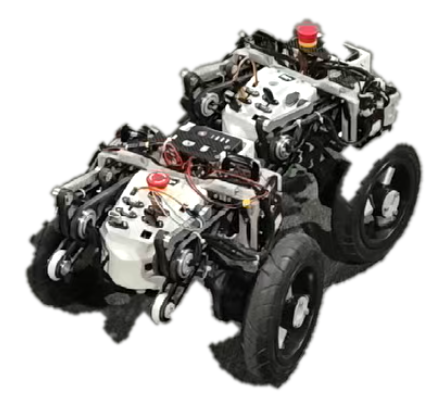
\includegraphics[width=0.70\textwidth]{images/robots/double_robot_cutout.png}
  \caption{自研链式轮足机器人实验平台实物}
  \label{fig:exp-robot-platform}
\end{figure}

硬件系统采用 Linux 主板与单片机协同的分层式架构。Linux 主板主要负责上层任务调度、链式运动学解算、UDP 通信、视觉铰接角解算、DMPC 优化求解和实验数据记录；单片机主要负责电机驱动、关节状态采集、惯性测量数据读取、底层 LQR 控制和执行器安全保护。上层控制器通过网络和串口等接口向底层控制器发送期望速度、期望角速度、腿长和控制模式等指令，底层控制器实时返回机体姿态、轮速、关节角、控制输入和故障状态等信息。

实验系统采集的数据主要包括机体俯仰角、角速度、轮端速度、腿长、关节角、控制力矩、UDP 通信时间戳、通信丢包情况、单目视觉铰接角解算结果以及链式系统的分布式跟踪误差。通过对上述数据进行同步记录和离线分析，可以从单体控制稳定性、通信可靠性、感知精度、链式运动学解算精度和优化控制效果等方面评价系统性能。

\section{实验方案与评价指标}
实验方案分为基础协同控制方案和优化协同控制方案两组。基础协同控制方案采用“分布式解算+LQR”的结构：上层根据链式运动学模型和铰接角信息逐级解算各单体期望速度，底层采用 LQR 控制器完成单体姿态稳定和速度跟踪。该组实验用于验证不引入预测优化和扰动补偿时，系统在通信、感知、分布式解算和基础跟踪控制方面的可实现性。

优化协同控制方案在基础方案上进一步引入 DMPC 和 ADRC。DMPC 用于在有限预测时域内协调链式系统的期望速度、航向角速度和铰接约束，ADRC 用于补偿单体等效受控系统中的模型误差和外部扰动。该组实验先比较未应用 ADRC 与应用 ADRC 后等效受控系统的预测误差，再验证同时应用 DMPC 和 ADRC 后链式系统的分布式跟踪误差变化。

具体实验采用分层数据流设计。上层 Linux 主板作为链式协同控制节点，按照固定控制周期采集本车状态、邻车状态和视觉铰接角信息，并通过分布式解算或 DMPC 生成单体期望速度与期望角速度；底层单片机接收上层参考量后执行 LQR 或 LQR-ADRC 控制，并将姿态、轮速、关节角和控制输入等状态量回传给上层。实验过程中同时记录上层计算结果、底层反馈数据和外部感知结果，便于对通信、感知、预测和跟踪误差进行离线对齐分析。

机器人之间的通信采用 UDP 方式实现。UDP 具有协议开销小、传输延迟低和实现简单等特点，适合链式机器人中高频状态广播和邻车信息交换。实验中每个数据包包含发送端编号、时间戳、序号、机体速度、航向角速度、姿态信息和控制模式等字段；接收端根据时间戳和序号统计通信延迟与丢包情况，并将最新有效邻车状态用于分布式运动学解算或 DMPC 预测优化。由于 UDP 不保证可靠传输，实验评价中需要单独统计丢包率和延迟，以分析通信不确定性对链式跟踪误差的影响。

相对定位采用单目视觉定位方式实现。实验中在相邻机器人或铰接机构相关位置布置标准二维码标记，单目摄像机识别二维码角点后，根据二维码实际尺寸、相机内参和透视投影关系求解标记相对于相机坐标系的位姿。进一步结合相机安装外参和机器人几何关系，可得到相邻单体之间的相对姿态和铰接角估计值。该方法结构简单、成本较低，适合在实验平台上提供铰接角观测；但其精度会受到图像分辨率、光照条件、运动模糊、二维码遮挡和相机标定误差影响，因此需要在实验中统计铰接角解算误差，并分析其对分布式解算结果的影响。

评价指标主要包括：单体 LQR 控制下的俯仰角误差、速度跟踪误差和稳定时间；UDP 通信丢包率与通信延迟；单目摄像机铰接角解算误差；链式系统分布式跟踪误差；等效受控系统预测误差；以及优化控制后链式系统跟踪误差的均值、最大值和收敛过程。上述指标分别对应底层稳定性、通信链路可靠性、感知精度、分布式解算精度和优化控制效果。

\section{基础协同控制方案实验结果}
基础协同控制方案首先验证单体 LQR 控制效果。实验中对单体机器人施加速度指令和姿态扰动，记录机体俯仰角、俯仰角速度、轮端速度、腿长和控制输入等数据。通过对姿态响应曲线和速度跟踪曲线进行分析，可以评价 LQR 控制器在偏置并联腿双轮足平台上的基本稳定能力、响应速度和稳态误差。

\begin{figure}[htbp]
  \centering
  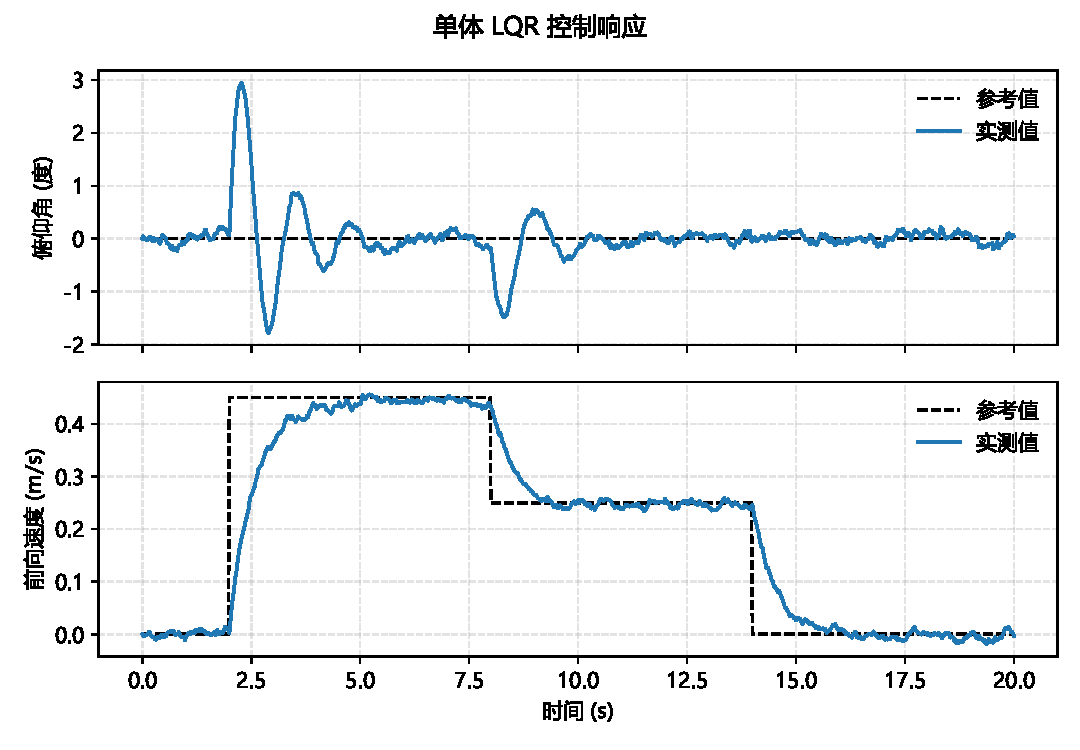
\includegraphics[width=0.92\textwidth]{images/experiment_results/fig5_lqr_single_control.pdf}
  \caption{单体 LQR 控制响应实验结果}
  \label{fig:exp-lqr-single-control}
\end{figure}

其次，对上层 Linux 主板与各单体控制器之间的 UDP 通信性能进行测试。实验记录数据包发送时间戳、接收时间戳和序号连续性，并统计通信丢包率与通信延迟。该实验用于评估分布式解算所依赖的数据链路是否能够满足链式系统实时控制要求。若通信延迟或丢包率较高，后车接收到的前车状态将出现滞后或缺失，从而影响铰接角解算和期望速度传播精度。

\begin{figure}[htbp]
  \centering
  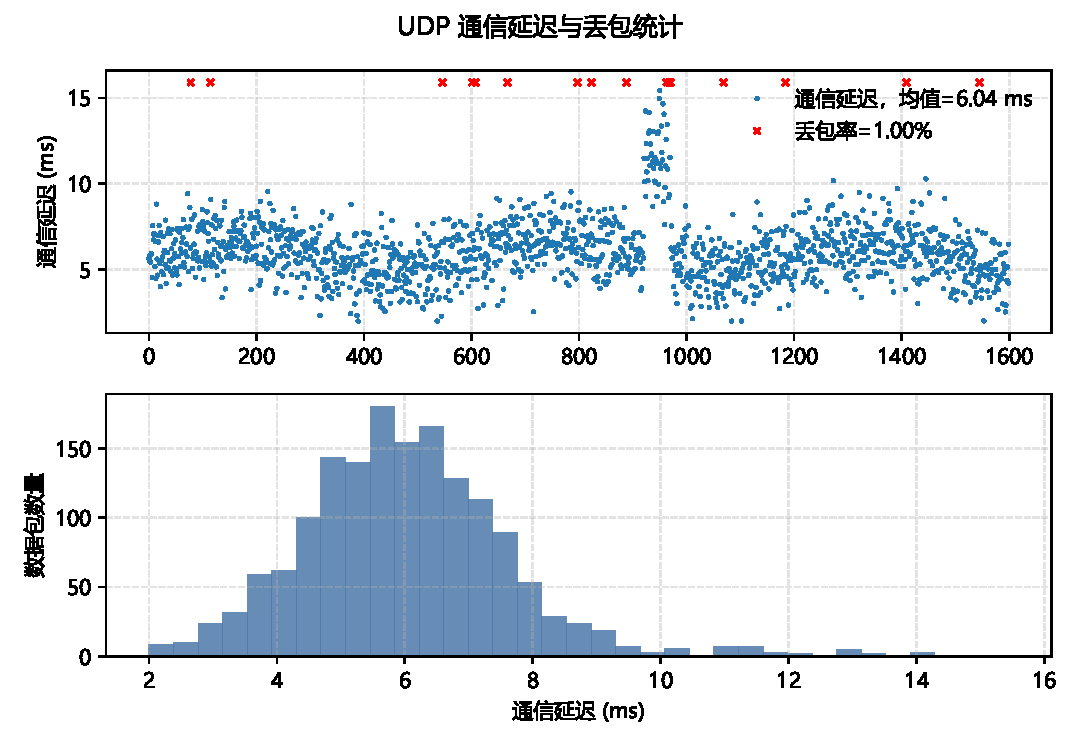
\includegraphics[width=0.92\textwidth]{images/experiment_results/fig5_udp_comm.pdf}
  \caption{UDP 通信延迟与丢包统计实验结果}
  \label{fig:exp-udp-comm}
\end{figure}

再次，对单目摄像机铰接角解算误差进行测试。实验中利用视觉算法估计相邻单体之间的铰接角，并与人工标定或参考测量结果进行对比，得到铰接角解算误差曲线和统计指标。铰接角是链式运动学分布式解算的关键输入，其测量误差会直接影响后续单体期望线速度和角速度的计算结果。

\begin{figure}[htbp]
  \centering
  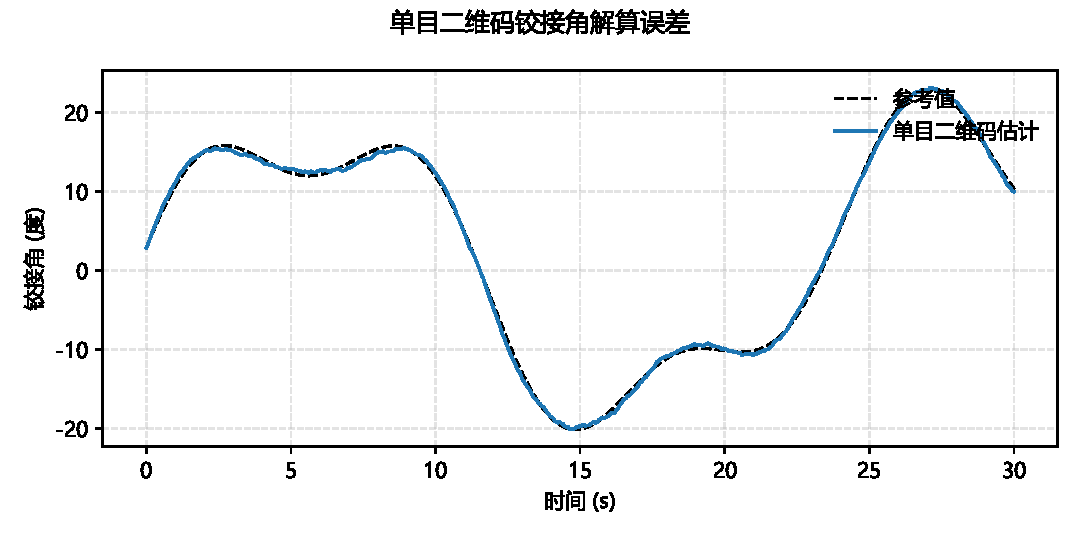
\includegraphics[width=0.92\textwidth]{images/experiment_results/fig5_vision_articulation_error.pdf}
  \caption{单目二维码铰接角解算误差实验结果}
  \label{fig:exp-vision-articulation}
\end{figure}

最后，在链式连接状态下测试分布式跟踪控制效果。头车接收期望速度和角速度指令，后续单体根据铰接角和前车状态逐级解算自身期望输入，并由底层 LQR 控制器执行。实验记录各单体速度、航向角速度、铰接角和链式构型误差，分析分布式解算与 LQR 控制组合下链式系统的跟踪误差。该结果作为后续优化协同控制方案的对照基准。

\begin{figure}[htbp]
  \centering
  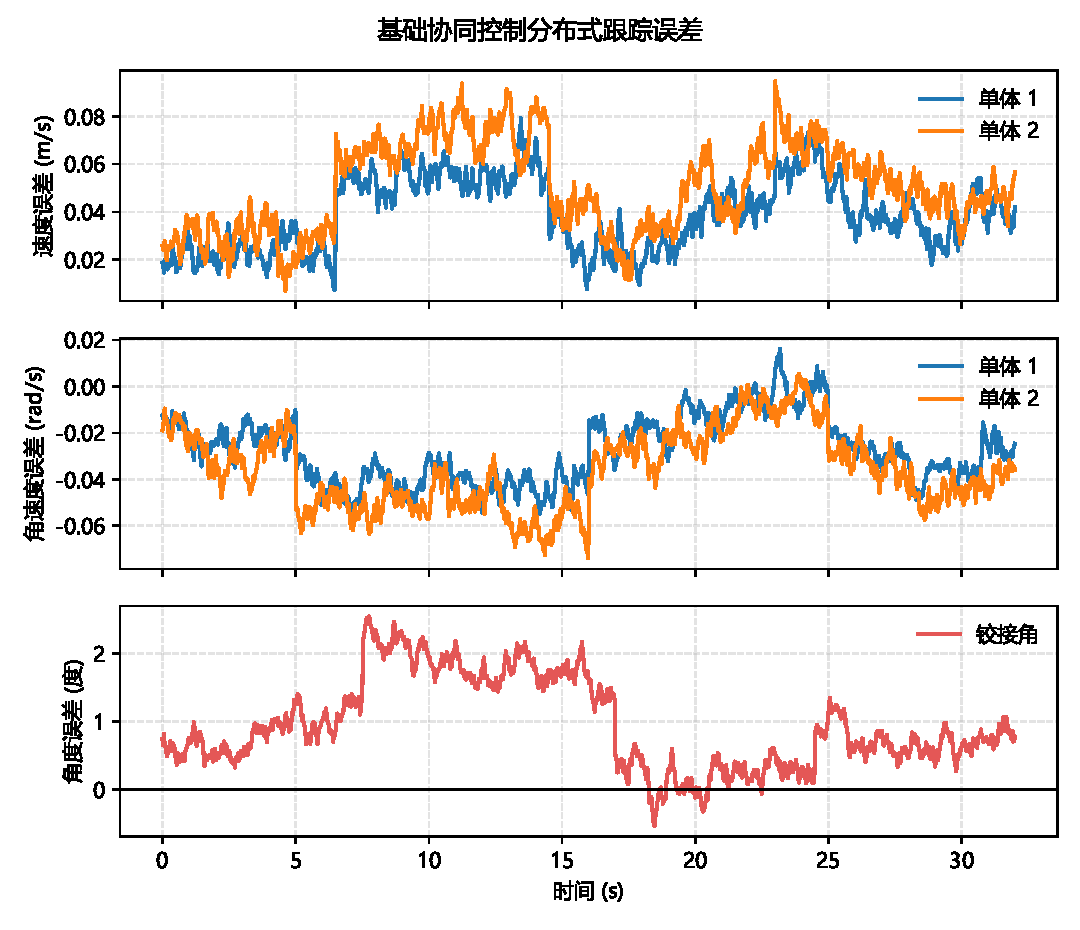
\includegraphics[width=0.92\textwidth]{images/experiment_results/fig5_chain_tracking_basic.pdf}
  \caption{基础协同控制分布式跟踪误差实验结果}
  \label{fig:exp-chain-tracking-basic}
\end{figure}

\FloatBarrier

\section{优化协同控制方案实验结果}
优化协同控制方案首先验证未应用 ADRC 时等效受控系统的预测误差。实验中保持基础 LQR 内环不变，将单体闭环系统近似为协同层的等效受控对象，并利用预测模型计算未来时域内的速度和角速度响应。将预测结果与实际测量结果对比，可以得到未补偿模型误差和外部扰动条件下的预测误差。该结果反映了仅依赖 LQR 闭环模型时，等效受控系统在实际平台上的模型偏差。

随后，在单体控制器中引入 ADRC 扰动补偿，并重新统计等效受控系统预测误差。ADRC 通过扩张状态观测器估计未建模动态、地面扰动和链式铰接耦合等总扰动，并在控制律中进行补偿。通过比较应用 ADRC 前后的预测误差曲线，可以评价扰动观测与补偿对等效受控模型一致性的改善效果。

\begin{figure}[htbp]
  \centering
  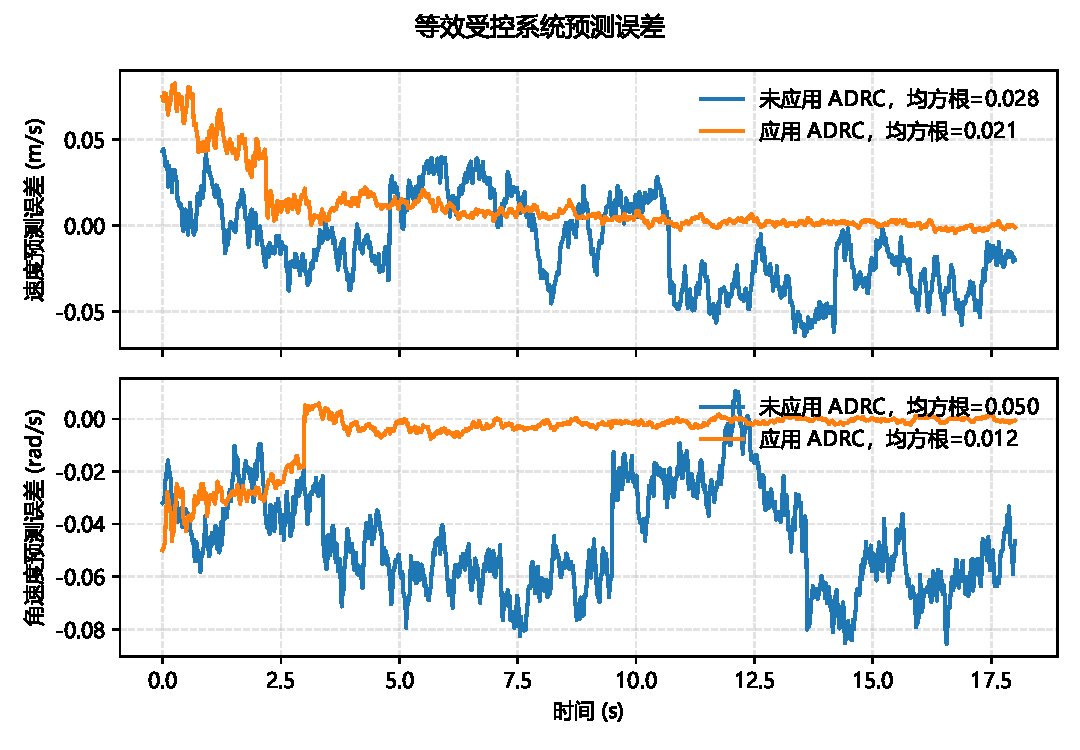
\includegraphics[width=0.92\textwidth]{images/experiment_results/fig5_prediction_error_adrc_compare.pdf}
  \caption{ADRC 引入前后等效受控系统预测误差对比}
  \label{fig:exp-prediction-adrc-compare}
\end{figure}

在完成等效受控系统验证后，进一步测试同时应用 DMPC 和 ADRC 的链式系统分布式跟踪效果。DMPC 根据当前状态、邻车预测信息和铰接约束生成更平滑的期望速度序列，ADRC 则提高底层单体对优化参考量的跟踪能力。实验记录各单体速度误差、角速度误差、铰接角误差和链式构型误差，并与基础协同控制方案结果进行对比。若优化方案有效，则应表现为分布式跟踪误差减小、铰接角波动降低以及链式运动过程更加平滑。

\begin{figure}[htbp]
  \centering
  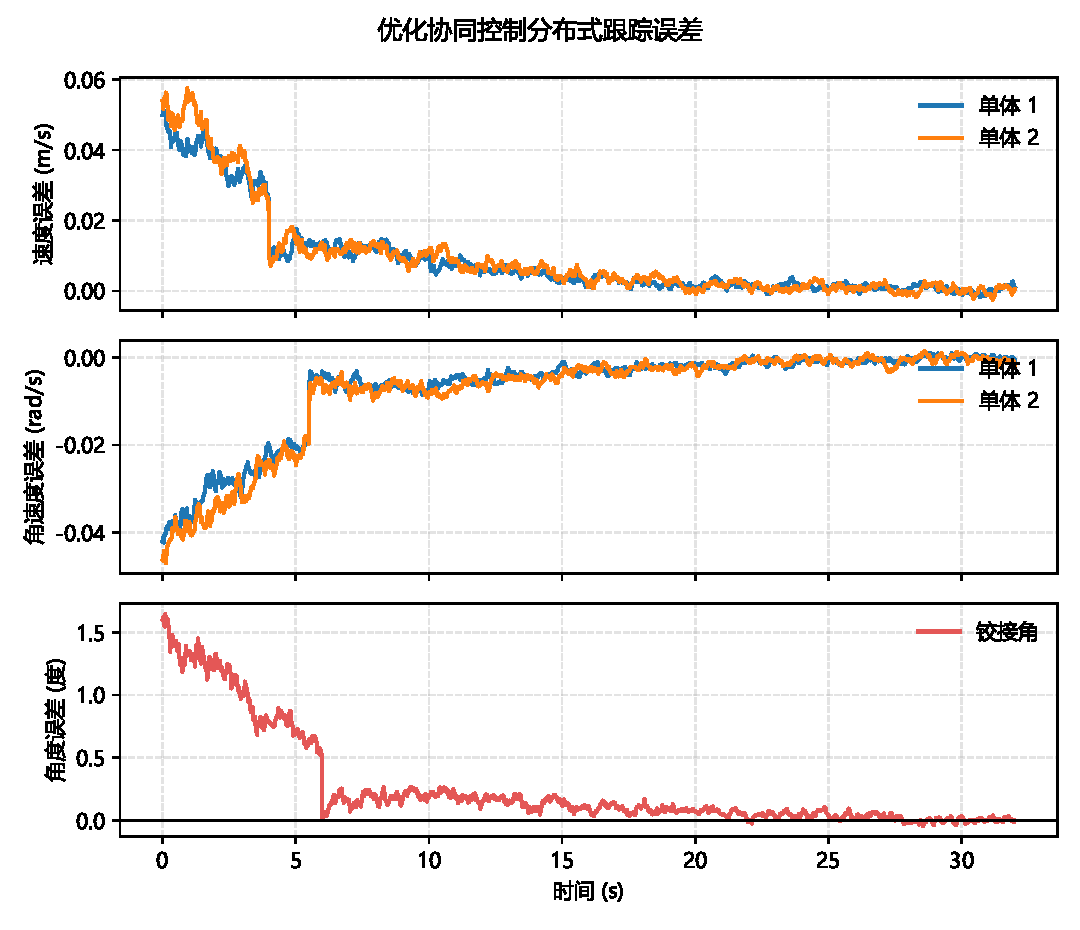
\includegraphics[width=0.92\textwidth]{images/experiment_results/fig5_chain_tracking_optimized.pdf}
  \caption{优化协同控制分布式跟踪误差实验结果}
  \label{fig:exp-chain-tracking-optimized}
\end{figure}

\begin{figure}[htbp]
  \centering
  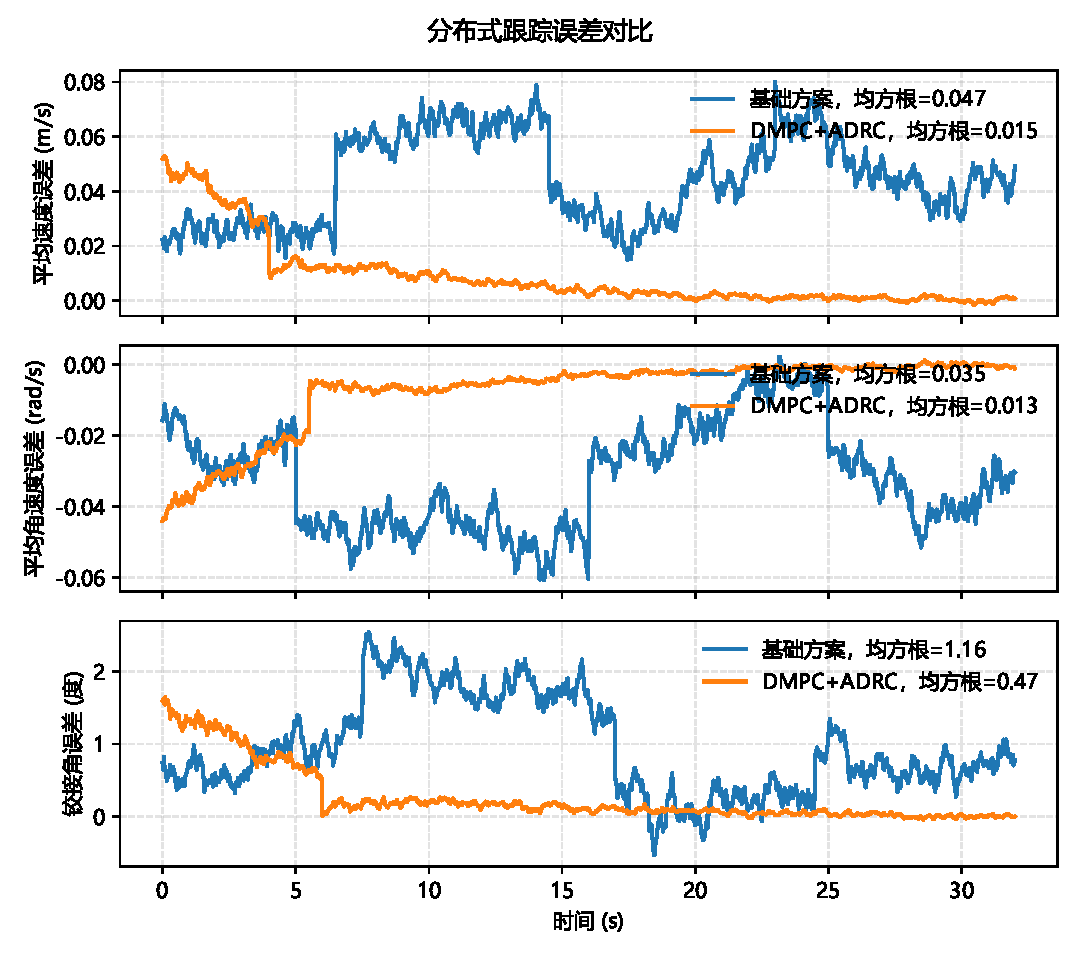
\includegraphics[width=0.92\textwidth]{images/experiment_results/fig5_tracking_error_compare.pdf}
  \caption{基础方案与优化方案分布式跟踪误差对比}
  \label{fig:exp-tracking-error-compare}
\end{figure}

\FloatBarrier

\section{本章小结}
本章围绕自研带铰接结构双轮足机器人平台，设计了基础协同控制方案和优化协同控制方案两组实验。基础方案重点验证 LQR 单体控制、UDP 通信性能、单目视觉铰接角解算和链式系统分布式跟踪效果；优化方案重点比较 ADRC 引入前后的等效受控系统预测误差，并进一步验证 DMPC 与 ADRC 共同作用下的链式系统跟踪性能。通过上述实验，可以从硬件平台、通信感知、基础控制和优化控制多个层面评价所提出协同控制方法的有效性。

% 后置内容
\backmatter

% 结论：在相应 TeX 文件撰写
%%
% BIThesis 本科毕业设计论文模板 —— 使用 XeLaTeX 编译 The BIThesis Template for Undergraduate Thesis
% This file has no copyright assigned and is placed in the Public Domain.
%%

\begin{conclusion}
  % 结论部分尽量不使用 \subsection 二级标题，只使用 \section 一级标题

  本文围绕自重组轮足机器人链式系统协同控制问题，开展了单体建模、平衡控制和链式协同运动建模研究。首先，针对单体轮腿机器人结构，建立了腿部运动学模型和虚拟模型控制映射关系，推导了腿部虚拟支撑力、摆杆力矩与关节驱动力矩之间的等效关系。其次，针对尾部辅助机构离地和触地两类典型工况，建立了单体动力学模型，并在平衡点附近线性化得到状态空间表达。在此基础上，设计了 LQR 状态反馈控制器，并通过参数化增益拟合方法提高控制器对腿长变化和构型变化的适应能力。

  针对链式系统协同运动问题，本文进一步分析了相邻单体之间的铰接几何约束，建立了由头车运动状态向后续单体逐级传播的运动学模型。基于该模型，构建了分层协同控制思路：上层根据链式几何约束生成各单体期望运动序列，下层利用单体平衡控制器实现稳定跟踪。该方法将链式协同运动问题与单体姿态稳定问题相分离，有助于降低控制器设计复杂度，并为后续引入 DMPC 约束优化提供了基础。

  后续研究将重点从三个方面继续完善：一是开展系统化实机实验，形成可量化的速度误差、姿态误差、稳定时间和控制输入对比结果；二是完善 DMPC 协同层，使其能够在预测时域内显式处理铰接角、速度和输入约束；三是进一步研究 LQR-ADRC 复合控制，通过扰动观测和补偿提升单体在模型误差、冲击载荷和复杂地形下的鲁棒性。
\end{conclusion}

% 参考文献：
% 添加文献时，请按 BibTeX 格式添加至 misc/ref.bib，并在正文所需位置使用 \cite{…} 引用。
% 如无特殊需要，无需改动相应 TeX 文件。
\input{misc/3_reference.tex}
% 附录：在相应 TeX 文件撰写；不需要时可删除
%%
% BIThesis 本科毕业设计论文模板 —— 使用 XeLaTeX 编译 The BIThesis Template for Undergraduate Thesis
% This file has no copyright assigned and is placed in the Public Domain.
%%

\begin{appendices}
  \section{主要符号说明}
  为便于阅读，本文使用的部分主要符号说明如下。$x,y$ 表示单体在世界坐标系下的位置；$\phi$ 表示单体航向角；$v$ 与 $\omega$ 分别表示单体线速度和角速度；$L_0$ 表示等效腿长；$\Phi_0$ 表示等效腿摆角；$\theta_i$ 表示链式系统中第 $i$ 个铰接角；$X$ 表示状态向量；$U$ 表示控制输入向量；$K$ 表示 LQR 反馈增益矩阵；$Q$ 与 $R$ 分别表示 LQR 性能指标中的状态权重矩阵和输入权重矩阵。

  \section{实验评价指标说明}
  链式自重组轮足机器人实验可采用以下指标进行评价：速度跟踪误差用于衡量单体对期望线速度和角速度的跟踪能力；姿态误差用于衡量机体俯仰角、滚转角和航向角的稳定性；铰接角误差用于衡量链式构型保持能力；控制输入峰值和控制输入变化率用于评价执行器负担和控制平滑性；稳定时间用于描述系统受到扰动或指令变化后的恢复速度。

\end{appendices}

% 致谢：在相应 TeX 文件撰写
%%
% BIThesis 本科毕业设计论文模板 —— 使用 XeLaTeX 编译 The BIThesis Template for Undergraduate Thesis
% This file has no copyright assigned and is placed in the Public Domain.
%%

% 致谢部分尽量不使用 \subsection 二级标题，只使用 \section 一级标题
\begin{acknowledgements}
  值此论文初稿完成之际，首先感谢导师在毕业设计选题、技术路线和论文写作方面给予的指导。自重组轮足机器人链式系统涉及机械结构、动力学建模、嵌入式实时控制、ROS 通信和实机调试等多个环节，每一部分的推进都离不开老师在方向把握和工程实现上的帮助。

  感谢实验室同学在机器人硬件调试、代码维护、实验平台搭建和问题讨论中给予的支持。项目代码从单体平衡控制逐步扩展到链式系统协同控制，期间积累了大量参数整定、通信调试和实车测试经验，这些工作为本文撰写提供了重要基础。

  最后感谢家人和朋友在毕业设计期间给予的理解与鼓励。后续工作仍需继续完善实验数据和控制策略，但这一阶段的整理让我对机器人系统设计、控制算法落地和工程文档写作有了更完整的认识。

  % 既然写到这里，那估计就要大功告成了。无论过程与结果如何，总是人生一段独特体验。祝贺！
  % 如有兴趣，可填写以下反馈问卷，帮助 BIThesis 未来优化。
  % https://wj.qq.com/s2/22532808/254f/
\end{acknowledgements}


\end{document}
